%
% Template Laporan Skripsi/Thesis
%
% @author  Andreas Febrian, Lia Sadita
% @version 1.03
%
% Dokumen ini dibuat berdasarkan standar IEEE dalam membuat class untuk
% LaTeX dan konfigurasi LaTeX yang digunakan Fahrurrozi Rahman ketika
% membuat laporan skripsi. Konfigurasi yang lama telah disesuaikan dengan
% aturan penulisan thesis yang dikeluarkan UI pada tahun 2008.
%

%
% Tipe dokumen adalah report dengan satu kolom.
%
\documentclass[12pt, a4paper, onecolumn, twoside, final]{report}
\raggedbottom

% Load konfigurasi LaTeX untuk tipe laporan thesis
\usepackage{uithesis}


% Load konfigurasi khusus untuk laporan yang sedang dibuat
%-----------------------------------------------------------------------------%
% Informasi Mengenai Dokumen
%-----------------------------------------------------------------------------%
%
% Judul laporan.
\var{\judul}{Implementing JSONField in Django}
%
% Tulis kembali judul laporan, kali ini akan diubah menjadi huruf kapital
\Var{\Judul}{Implementing JSONField in Django}
%
% Tulis kembali judul laporan namun dengan bahasa Ingris
\var{\judulInggris}{Implementing JSONField in Django}
%
% Tulis judul dalam bahasa Indonesia
\var{\judulIndonesia}{Implementasi JSONField pada Django}

%
% Tipe laporan, dapat berisi Skripsi, Tugas Akhir, Thesis, atau Disertasi
\var{\type}{Bachelor Thesis}
%
% Tulis kembali tipe laporan, kali ini akan diubah menjadi huruf kapital
\Var{\Type}{Bachelor Thesis}
%
% Tulis nama penulis
\var{\penulis}{Sage Muhammad Abdullah}
%
% Tulis kembali nama penulis, kali ini akan diubah menjadi huruf kapital
\Var{\Penulis}{Sage Muhammad Abdullah}
%
% Tulis NPM penulis
\var{\npm}{1706979455}
%
% Tuliskan Fakultas dimana penulis berada
\var{\fakultas}{Computer Science}
\Var{\Fakultas}{Computer Science}
%
% Tuliskan Program Studi yang diambil penulis
\var{\program}{Computer Science Undergraduate}
\Var{\Program}{Computer Science Undergraduate}
%
% Tuliskan Program Studi dalam bahasa Indonesia
\var{\programIndonesia}{Ilmu Komputer}
\Var{\ProgramIndonesia}{Ilmu Komputer}
%
% Tuliskan kota/kabupaten publikasi laporan
\var{\kota}{Depok}
\Var{\Kota}{Depok}
%
% Tuliskan tahun publikasi laporan
\Var{\bulanTahun}{January 2021}
%
% Tuliskan gelar yang akan diperoleh dengan menyerahkan laporan ini
\var{\gelar}{S.Kom.}
%
% Tuliskan tanggal pengesahan laporan, waktu dimana laporan diserahkan ke
% penguji/sekretariat
\var{\tanggalSiapSidang}{01 November 2020}
%
% Tuliskan tanggal keputusan sidang dikeluarkan dan penulis dinyatakan
% lulus/tidak lulus
\var{\tanggalLulus}{11 January 2021}
% Tuliskan tanggal pengesahan laporan final, waktu dimana laporan
% diserahkan ke perpustakaan
\var{\tanggalFinal}{11 January 2021}
%
% Tuliskan pembimbing
\var{\pembimbingSatu}{Dr. Ade Azurat}
\var{\pembimbingDua}{Hafiyyan Sayyid Fadhlillah, M.Kom., S.Kom.}
%
% Tuliskan penguji
\var{\pengujiSatu}{Penguji Pertama Anda}
\var{\pengujiDua}{Penguji Kedua Anda}

% Tulisan untuk menandakan halaman lampiran lanjutan
\var{\continued}{(continued)}

%-----------------------------------------------------------------------------%
% Judul Setiap Bab
%-----------------------------------------------------------------------------%
%
% Berikut ada judul-judul setiap bab.
% Silahkan diubah sesuai dengan kebutuhan.
%
\Var{\kataPengantar}{Preface}
\Var{\babSatu}{Introduction}
\Var{\babDua}{Django Web Framework}
\Var{\babTiga}{Problem Analysis}
\Var{\babEmpat}{Implementation}
\Var{\babLima}{Results and Evaluation}
\Var{\kesimpulan}{Conclusions}

% Daftar pemenggalan suku kata dan istilah dalam LaTeX
%
% Hyphenation untuk Indonesia 
%
% @author  Andreas Febrian
% @version 1.00
% 
% Tambahkan cara pemenggalan kata-kata yang salah dipenggal secara otomatis 
% oleh LaTeX. Jika kata tersebut dapat dipenggal dengan benar, maka tidak 
% perlu ditambahkan dalam berkas ini. Tanda pemenggalan kata menggunakan 
% tanda '-'; contoh:
% menarik
%   --> pemenggalan: me-na-rik
%

\hyphenation{
    % alphabhet A
    a-na-li-sa a-tur 
    a-pli-ka-si 
    % alphabhet B
    ba-ngun-an 
    be-be-ra-pa 
    ber-ge-rak
    ber-ke-lan-jut-an 
    ber-pe-nga-ruh 
    % alphabhet C
    ca-ri
    % alphabhet D
    di-da-pat-kan di-sim-pan di-pim-pin de-ngan da-e-rah di-ba-ngun da-pat di-nya-ta-kan 
    di-sim-bol-kan di-pi-lih di-li-hat de-fi-ni-si di-de-fi-ni-si-kan di-mi-li-ki
    % alphabhet E
    e-ner-gi eks-klu-sif
    % alphabhet F
    fa-si-li-tas
    % alphabhet G
    ga-bung-an ge-rak
    % alphabhet H
    ha-lang-an
    % alphabhet I
    % alphabhet J
    % alphabhet K
    ke-hi-lang-an
    ku-ning 
    kua-li-tas ka-me-ra ke-mung-kin-an ke-se-pa-ham-an
    % alphabhet L
    ling-kung-an
    % alphabhet M
    me-neng-ah
    meng-a-tas-i me-mung-kin-kan me-nge-na-i me-ngi-rim-kan 
    meng-u-bah meng-a-dap-ta-si me-nya-ta-kan mo-di-fi-ka-si
    meng-a-tur meng-a-rah-kan mi-lik
    % alphabhet N
    nya-ta non-eks-klu-sif
    % alphabhet O
    % alphabhet P
	pe-nye-rap-an 
	pe-ngon-trol
    pe-mo-del-an
    pe-ran  pe-ran-an-nya
    pem-ba-ngun-an pre-si-den pe-me-rin-tah prio-ri-tas peng-am-bil-an 
    peng-ga-bung-an pe-nga-was-an pe-ngem-bang-an 
    pe-nga-ruh pa-ra-lel-is-me per-hi-tung-an per-ma-sa-lah-an 
    pen-ca-ri-an peng-struk-tur-an pen-ting pen-ting-nya
    % alphabhet Q
    % alphabhet R
    ran-cang-an
    % alphabhet S
    si-mu-la-si sa-ngat
    % alphabhet T
    te-ngah
    ter-da-pat
    % alphabhet U
    % alphabhet V
    va-ri-an va-ri-a-si
    % alphabhet W
    % alphabhet X
    % alphabhet Y
    % alphabhet Z
    % special
}

\hyphenation{
	Committee
	PostgreSQL
	MariaDB
	MySQL
	Psycopg
}
% Daftar istilah yang mungkin perlu ditandai
%
% @author  Andreas Febrian
% @version 1.00
%
% Mendaftar seluruh istilah yang mungkin akan perlu dijadikan
% italic atau bold pada setiap kemunculannya dalam dokumen.
%

\var{\license}{\f{Creative Commons License 1.0 Generic}}
\var{\bslash}{$\setminus$}


% Awal bagian penulisan laporan
\begin{document}

%
% Sampul Laporan
%
% Sampul Laporan

%
% @author  unknown
% @version 1.01
% @edit by Andreas Febrian
%

\begin{titlepage}
    \begin{center}
        \begin{figure}
            \begin{center}
                
\includegraphics[width=2.5cm]{pics/makara_kuning.png}
            \end{center}
        \end{figure}
        \vspace*{0cm}
        \bo{
        	UNIVERSITAS INDONESIA\\
        }

        \vspace*{1.0cm}
        % judul thesis harus dalam 14pt Times New Roman
        \bo{\Judul} \\[1.0cm]

        \vspace*{2.5 cm}
        % harus dalam 14pt Times New Roman
        \bo{\Type}

        \vspace*{3 cm}
        % penulis dan npm
        \bo{\Penulis} \\
        \bo{\npm} \\

        \vspace*{5.0cm}

        % informasi mengenai fakultas dan program studi
        \bo{
        	FAKULTAS \Fakultas\\
        	PROGRAM STUDI \Program \\
        	DEPOK \\
        	\bulanTahun
        }
    \end{center}
\end{titlepage}

\forceclearchapter

%
% Gunakan penomeran romawi
\pagenumbering{roman}
\pagestyle{first-pages}

%
% load halaman judul dalam
\addChapter{COVER SHEET}
%
% Halaman Judul Laporan
%
% @author  unknown
% @version 1.01
% @edit by Andreas Febrian
%

\begin{titlepage}
    \begin{center}\begin{figure}
            \begin{center}
                
\includegraphics[width=2.5cm]{pics/makara.png}
            \end{center}
        \end{figure}
        \vspace*{0cm}
        \bo{
        	UNIVERSITAS INDONESIA\\
        }

        \vspace*{1.0cm}
        % judul thesis harus dalam 14pt Times New Roman
        \bo{\Judul} \\[1.0cm]

        \vspace*{2.5 cm}
        % harus dalam 14pt Times New Roman
        \bo{\Type} \\
        % keterangan prasyarat
        \bo{Diajukan sebagai salah satu syarat untuk memperoleh gelar \\
        \gelar}\\

        \vspace*{3 cm}
        % penulis dan npm
        \bo{\Penulis} \\
        \bo{\npm} \\

        \vspace*{5.0cm}

        % informasi mengenai fakultas dan program studi
        \bo{
        	FAKULTAS \Fakultas\\
        	PROGRAM STUDI \Program \\
        	DEPOK \\
        	\bulanTahun
        }
    \end{center}
\end{titlepage}

\forceclearchapter

%
% setelah bagian ini, halaman dihitung sebagai halaman ke 2
\setcounter{page}{2}

%
% load halaman pengesahan
\addChapter{APPROVAL SHEET}
%
% Halaman Pengesahan
%
% @author  Andreas Febrian
% @version 1.01
%

\chapter*{HALAMAN PERSETUJUAN}

\vspace*{0.2cm}
\noindent

\noindent
\begin{tabular}{l l p{11cm}}
	\bo{Judul}&: & \judul \\
	\bo{Nama}&: & \penulis \\
	\bo{NPM}&: & \npm \\
\end{tabular} \\

\vspace*{1.2cm}

\noindent Laporan \type~ini telah diperiksa dan disetujui.\\[0.3cm]
\begin{center}
\tanggalFinal \\[2cm]
\end{center}

\begin{center}
\begin{multicols}{2}
\underline{\pembimbingSatu}\\[0.1cm]
Pembimbing \type

\underline{\pembimbingDua}\\[0.1cm]
Pembimbing \type
\end{multicols}
\end{center}

\newpage

\forceclearchapter
%
% load halaman orisinalitas
\addChapter{ORIGINALITY STATEMENT SHEET}
%
% Halaman Orisinalitas
%
% @author  Andreas Febrian
% @version 1.01
%

\chapter*{\uppercase{halaman pernyataan orisinalitas}}
\vspace*{2cm}

\begin{center}
	\bo{\type~ini adalah hasil karya saya sendiri, \\
	dan semua sumber baik yang dikutip maupun dirujuk \\
	telah saya nyatakan dengan benar.} \\
	\vspace*{2.6cm}

	\begin{tabular}{l c l}
	\bo{Nama} & : & \bo{\penulis} \\
	\bo{NPM} & : & \bo{\npm} \\
	\bo{Tanda Tangan} & : & \\
	& & \\
	& & \\
	\bo{Tanggal} & : & \bo{\tanggalSiapSidang} \\
	\end{tabular}
\end{center}

\newpage

\forceclearchapter
%
%
\addChapter{VALIDATION SHEET}
%
% Halaman Pengesahan Sidang
%
% @author  Andreas Febrian, Andre Tampubolon
% @version 1.02
%

\chapter*{HALAMAN PENGESAHAN}

\vspace*{0.4cm}
\noindent

\noindent
\begin{tabular}{ll p{9cm}}
	\type~ini diajukan oleh&: & \\
	Nama&: & \penulis \\
	NPM&: & \npm \\
	Program Studi&: & \program \\
	Judul \type&: & \judul \\
\end{tabular} \\

\vspace*{1.0cm}

\noindent \bo{Telah berhasil dipertahankan di hadapan Dewan Penguji
dan diterima sebagai bagian persyaratan yang diperlukan untuk
memperoleh gelar \gelar~pada Program Studi \program, Fakultas
\fakultas, Universitas Indonesia.}\\[0.2cm]

\begin{center}
	\bo{DEWAN PENGUJI}
\end{center}

\vspace*{0.3cm}

\begin{tabular}{l l l l }
	& & & \\
	Pembimbing 1&: & \pembimbingSatu & (\hspace*{3.0cm}) \\
	& & & \\
	Pembimbing 2&: & \pembimbingDua & (\hspace*{3.0cm}) \\
	& & & \\
	Penguji 1&: & \pengujiSatu & (\hspace*{3.0cm}) \\
	& & & \\
	Penguji 2&: & \pengujiDua & (\hspace*{3.0cm}) \\
\end{tabular}\\

\vspace*{2.0cm}

\begin{tabular}{ll l}
	Ditetapkan di&: & Depok\\
	Tanggal&: & \tanggalLulus \\
\end{tabular}


\newpage

\forceclearchapter
%
%
\addChapter{STATEMENT OF APPROVAL FOR ACADEMIC PUBLICATION}
%
% @author  Andre Tampubolon, Andreas Febrian
% @version 1.01
%

\chapter*{\uppercase{
	Statement of Approval
	for Academic Publication}}

\vspace*{0.2cm}
\noindent
As a \f{civitas academica} of Universitas Indonesia, I the undersigned:
\vspace*{0.4cm}


\begin{tabular}{p{4.2cm} l p{6cm}}
	\bo{Name} & : & \penulis \\
	\bo{NPM} & : & \npm \\
	\bo{Program} & : & \program\\
	\bo{Faculty} & : & \fakultas\\
	\bo{Type of Work} & : & \type \\
\end{tabular}

\vspace*{0.6cm}
\noindent for the development of science, approve to give my work titled:
\begin{center}
	\judul
\end{center}
and its resources to Universitas Indonesia under a \bo{non-exclusive,
royalty-free license}. With the license, Universitas Indonesia has the
right to store, adapt, manage in the form of a database, take care of,
and publish my work as long as my name is included as the writer/creator
and as the copyright owner.\\

\begin{center}
	\vspace*{0.8cm}
	\begin{tabular}{lll}
		Written in&: & Depok \\
		On&: & \tanggalSiapSidang \\
	\end{tabular}\\

	\vspace*{0.5cm}
	The proponent \\
	\vspace*{1.25cm}
	(\penulis)
\end{center}

\newpage

\forceclearchapter
%
%
\addChapter{\kataPengantar}
%-----------------------------------------------------------------------------%
\chapter*{\kataPengantar}
%-----------------------------------------------------------------------------%

Template ini disediakan untuk orang-orang yang berencana menggunakan \latex~untuk membuat dokumen tugas akhir.
\todo{Silakan ganti pesan ini dengan pendahuluan kata pengantar Anda.}

Ucapan Terima Kasih:
\begin{enumerate}[topsep=0pt,itemsep=-1ex,partopsep=1ex,parsep=1ex]
	\item Pembimbing.
	\item Dosen.
	\item Instansi.
	\item Orang tua.
	\item Sahabat.
	\item Teman.
\end{enumerate}

Penulis menyadari bahwa laporan \type~ini masih jauh dari sempurna. Oleh karena itu, apabila terdapat kesalahan atau kekurangan dalam laporan ini, Penulis memohon agar kritik dan saran bisa disampaikan langsung melalui \f{e-mail} \code{emailanda@mail.id}.

\begin{figure}
	\centering
	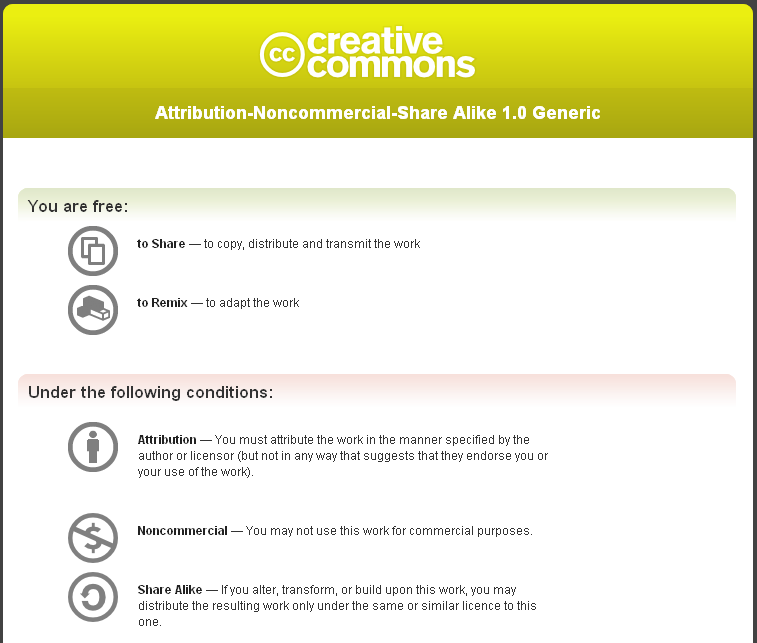
\includegraphics[width=0.74\textwidth]
	{pics/creative_commons.png}
	\caption{\license}
	\label{fig:lisensi}
\end{figure}

Terkait template ini, \pic~\ref{fig:lisensi} diambil dari \url{http://creativecommons.org/licenses/by-nc-sa/1.0/deed.en_CA}. Jika ingin mengentahui lebih lengkap mengenai \license, silahkan buka \url{http://creativecommons.org/licenses/by-nc-sa/1.0/legalcode}.
Seluruh dokumen yang dibuat dengan menggunakan template ini sepenuhnya menjadi hak milik pembuat dokumen dan bebas didistribusikan sesuai dengan keperluan masing-masing.
Lisensi hanya berlaku jika ada orang yang membuat template baru dengan menggunakan template ini sebagai dasarnya.

Penyusun template ingin berterima kasih kepada Andreas Febrian, Lia Sadita, Fahrurrozi Rahman, Andre Tampubolon, dan Erik Dominikus atas kontribusinya dalam template yang menjadi pendahulu template ini.
Penyusun template juga ingin mengucapkan terima kasih kepada Azhar Kurnia atas kontribusinya dalam template yang menjadi pendahulu template ini.

Semoga template ini dapat membantu orang-orang yang ingin mencoba menggunakan \latex.
Semoga template ini juga tidak berhenti disini dengan ada kontribusi dari para penggunanya.
Jika Anda memiliki perubahan yang dirasa penting untuk disertakan dalam template, silakan lakukan \f{fork} repositori Git template ini di \url{https://gitlab.com/ichlaffterlalu/latex-skripsi-ui-2017}, lalu lakukan \f{merge request} perubahan Anda terhadap \f{branch} \code{master}.
Kami berharap agar \f{template} ini dapat terus diperbarui mengikuti perubahan ketentuan dari pihak Rektorat Universitas Indonesia, dan hal itu tidak mungkin terjadi tanpa kontribusi dari teman-teman sekalian.

\vspace*{0.1cm}
\begin{flushright}
Depok, \tanggalSiapSidang\\[0.1cm]
\vspace*{1cm}
\penulis

\end{flushright}

%
%
\fancypagestyle{plain}{
	\fancyhead{}
	\fancyfoot[C]{\thepage}
	\fancyfoot[R]{\footnotesize \fontfamily{phv} \selectfont \bo{Universitas Indonesia}}
}
\addChapter{ABSTRACT}
%
% Halaman Abstract
%
% @author  Andreas Febrian
% @version 1.00
%

\chapter*{Abstract}
\singlespacing

\vspace*{0.2cm}

\noindent \begin{tabular}{l l p{11.0cm}}
	Name&: & \penulis \\
	Program&: & \program \\
	Title&: & \judulInggris \\
\end{tabular} \\

\vspace*{0.5cm}

\noindent
In web development, it is a common practice to use a web framework to build web
applications. One of the most popular web frameworks is Django, a free and
open-source web framework written in Python. Among the wide range of features
in Django, the object-relational mapping (ORM) system is the most complex. The
ORM system in Django maps data models to relational database tables. The data
models are defined as Python classes that have attributes known as model
fields. One of the model fields available in Django is \verb|JSONField| that
allows programmers to store and query semi-structured data using the JSON data
format in a relational database. Before this research, \verb|JSONField| was
only available for the PostgreSQL database system. Meanwhile, Django officially
supports PostgreSQL, MariaDB, MySQL, SQLite, and Oracle Database. This research
aimed to implement a new \verb|JSONField| that is compatible with all database
systems supported by Django. The implementation was created as part of the
Google Summer of Code 2019 program and was merged into the Django codebase for
the release of Django 3.1. In addition to the implementation, this research
also covers some examples of \verb|JSONField| usage with Django's built-in
model validation feature to validate the JSON data in a \verb|JSONField|.\\

\vspace*{0.2cm}

\noindent \bo{Keywords:} \\
\verb|JSONField|, JSON, Django, database, object-relational mapping,
semi-structured data \\

\onehalfspacing
\newpage

%
%
%
% Halaman Abstrak
%
% @author  Andreas Febrian
% @version 1.00
%

\chapter*{Abstrak}
\singlespacing

\vspace*{0.2cm}

\noindent \begin{tabular}{l l p{10cm}}
	Name&: & \penulis \\
	Program Studi&: & \programIndonesia \\
	Judul&: & \judulIndonesia \\
\end{tabular} \\

\vspace*{0.5cm}

\noindent
Skripsi ini menjelaskan tentang implementasi dan analisis JSONField pada
\f{framework} web Django. JSONField memungkinkan penggunanya untuk menyimpan
dan mencari data semi-terstruktur dalam basis data relasional dengan
memanfaatkan alat \f{object-relational mapping} yang ada pada Django.
Implementasi ini harus memperhitungkan kompatibilitas dengan semua sistem basis
data yang didukung secara resmi oleh Django, yakni PostgreSQL, SQLite, MySQL,
MariaDB, dan Oracle Database. Implementasi ini dibuat sebagai bagian dari
program Google Summer of Code 2019 dan telah digabungkan ke dalam basis kode
Django untuk perilisan Django 3.1. Selain itu, skripsi ini juga membahas
analisis penggunaan JSONField dengan fitur validasi model yang ada pada Django
untuk memvalidasi data JSON, serta tolok ukur penggunaan JSONField dengan data
uji. \\

\vspace*{0.2cm}

\noindent \bo{Kata kunci:} \\
JSONField, JSON, Django, basis data, \f{object-relational mapping}, data
semi-terstruktur \\

\onehalfspacing
\newpage


%
% Daftar isi, gambar, tabel, dan kode
%
\phantomsection %hack to make them clickable
\singlespacing
\tableofcontents
\onehalfspacing
\clearpage
\phantomsection %hack to make them clickable
\singlespacing
\listoffigures
\onehalfspacing
\clearpage
\phantomsection %hack to make them clickable
\singlespacing
\listoftables
\onehalfspacing
\clearpage
\phantomsection %hack to make them clickable
\addcontentsline{toc}{chapter}{\lstlistlistingname}
\singlespacing
\lstlistoflistings
\onehalfspacing

% Jika penomoran romawi selesai di ganjil
% \naiveoddclearchapter
% Jika penomoran romawi selesai di genap
\naiveevenclearchapter

%
% Gunakan penomeran Arab (1, 2, 3, ...) setelah bagian ini.
%
\pagenumbering{arabic}
\pagestyle{standard}
% \setlength{\belowcaptionskip}{+2pt}


\setoddevenheader
%-----------------------------------------------------------------------------%
\chapter{\babSatu}
%-----------------------------------------------------------------------------%

This chapter explains the background of this research and the problem to be
solved by this research.

%-----------------------------------------------------------------------------%
\section{Research Background}
%-----------------------------------------------------------------------------%

When the web platform was in its early stages, every part of a web application
was programmed without the help of a web framework. At that time, developing a
web application required extensive knowledge of how the web works. Depending on
the web application, the programmers might need deep understanding of the
Hypertext Transfer Protocol (HTTP), the Hypertext Markup Language (HTML), and
other things such as databases. If the web application was not programmed
correctly, it could lead to a lot of errors and security holes in the web
application.

Web frameworks aim to solve this problem by providing a standard way to build
web applications. Web frameworks help eliminate the overhead of implementing
common parts of web applications such as the HTTP layer, the user interface
layer, and the database layer. By using a web framework, programmers can build
web applications more quickly and safely by focusing more on the business logic
of the web application itself instead of the more intricate details.

Among the widely-used web frameworks is Django, a free and open-source web
framework written in Python.\footnote{\url{https://djangoproject.com}} Django
encourages rapid development and clean, pragmatic design \cite{django}. Django
was designed to help developers build their website quickly and securely with
scalability in mind.

One of the main features of Django is an object-relational mapping (ORM) tool
in the database layer \cite{django}. Django's ORM tool provides an
object-oriented abstraction of the database by mapping data models (represented
as Python classes) to tables in a relational database. The columns of a
database table are defined as attributes (called fields) inside the model
class. Using Django's ORM tool, programmers can interact with the database by
writing Python code instead of writing Structured Query Language (SQL)
statements. The abstraction provided by Django's ORM tool also helps
programmers avoid common mistakes that can lead to security issues such as SQL
injections.

Relational database systems can be used to manage structured data in the form
of tables with strict standards. The tables in a relational database can be
linked (related) based on data that is common to each table. Relating the
tables is possible because relational database systems enforce the data to be
consistent with a defined schema. This consistency is implemented according to
the Atomicity, Consistency, Isolation, and Durability (ACID) properties of
relational database transactions \cite{abramova_nosql}. These properties
guarantee that the data is valid despite any events of power failures, errors,
and other accidents.

Meanwhile, there has been an increase in the popularity of non-relational
databases, commonly known as NoSQL databases \cite{paul_nosql}. NoSQL
encourages the simplicity of database design, which makes the process of
scaling the database to multiple clusters of machines easier
\cite{leavitt_nosql}. Instead of tables, most NoSQL databases store data in the
form of key-value stores, document stores, or graphs \cite{strauch_nosql}.
NoSQL databases are also considered as more flexible due to its dynamic schema.
For example, some document-based NoSQL databases store data in JavaScript
Object Notation (JSON) format, which means that the schema is defined in the
data itself.

However, NoSQL databases also have their own downsides. Most NoSQL databases do
not fully support the ACID principles found in relational databases
\cite{cattell_nosql}. Instead of the ACID principles, they focus on the
Basically Available, Soft state, and Eventually consistent (BASE) principles
\cite{abramova_nosql}. The BASE principles state that the data should be
available most of the time (it can support partial failures), the data does not
have to be consistent at all times (soft state), but the data is guaranteed to
be consistent at some point (eventually). In addition, they also lack the
ability to perform joins across tables due to their horizontal data
distribution \cite{pokorny_nosql} and the use of denormalized data, which makes
it harder to deal with entity relations.

To compete with NoSQL databases, some relational database systems have come up
with their own ways to provide more flexibility for the data model. Some of
them provide the option to combine structured data with some form of
semi-structured data, most commonly in JSON format \cite{mariadb_json}. On
these databases, the user can store JSON data in a table column. This
combination gives all the benefits of using a relational database, while still
allowing the simplicity and flexibility of semi-structured data.

From version 1.9 until version 3.0, Django had provided an implementation of
\code{JSONField}. However, it was exclusively available for PostgreSQL. This
\code{JSONField} allowed its users to store and query JSON data in a relational
database column using the \code{jsonb} data type found only on PostgreSQL at
the time.\footnote{PostgreSQL has two JSON data types: \code{json} and
\code{jsonb}. Django's \code{JSONField} uses \code{jsonb}.} Django officially
supports PostgreSQL, SQLite, MySQL, MariaDB, and Oracle Database backends. Over
the years since the initial PostgreSQL \code{JSONField} implementation, those
database systems have developed their own support for managing JSON data.
However, Django had yet to implement \code{JSONField} for database backends
other than PostgreSQL.

The limited support for \code{JSONField} prompted the Django community to
create their own \code{JSONField} implementations for other database backends.
Some of them target one specific database backend and utilize various functions
provided by the database system to add extended querying capabilities
\cite{mysql_jsonfield, oracle_jsonfield}. Some other implementations
focus on cross-database support, thus they are only implemented as text-based
fields that do not have any extended querying capabilities
\cite{ryan_jsonfield}.

The individual efforts for implementing \code{JSONField} result in the
abundance of third-party \code{JSONField} packages on PyPI.\footnote{The Python
Package Index (PyPI) is a software repository for the Python programming
language.} Some of them are very popular, such as the \mbox{jsonfield} package
that has more than 1100 stars on GitHub \cite{ryan_jsonfield}. While this
indicates a popular demand for \code{JSONField}, it also indicates a
fragmentation problem as people use different \code{JSONField} packages. Thus,
there's a motivation to bring \code{JSONField} into Django's core model fields.

There's also a motivation to implement additional validations for JSON data in
a \code{JSONField}. By default, the validation for JSON data on the database
level only validates the syntax and not the information contained in the data
iself. Meanwhile, the flexibility of JSON data in a \code{JSONField} might
introduce invalid information or abnormalities within the data. For example,
the data might refer to a nonexisting record in one of the database tables. To
ensure the correctness of \code{JSONField} data, additional validations need to
be implemented.

In addition, recent studies showed interest in measuring the performance of
relational databases in handling JSON data. Relational databases are not
dedicated for storing JSON data, thus they may not perform well compared to
NoSQL databases. However, recent benchmarks by EnterpriseDB showed that
PostgreSQL outperformed MongoDB in varied workloads with JSON data
\cite{enterprisedb_benchmark}.\footnote{MongoDB is one of the most popular
document-oriented NoSQL database systems.} Some extensive benchmarks on
PostgreSQL, MySQL, and MongoDB also showed that the performance differences
were not significant, especially for smaller documents \cite{dolgov_benchmark}.
However, these benchmarks were done directly on the database systems instead of
using an ORM tool. Therefore, further studies of relational databases'
performance in handling JSON data using an ORM tool would provide new insights
on this topic.

With the motivations described in the previous paragraphs, this research aimed
to implement \code{JSONField} in Django, demonstrate additional validations for
\code{JSONField}, and provide an analysis of \code{JSONField} performance. The
new implementation of \code{JSONField} would have cross-database support,
extended querying support, and compatibility with the previous \code{JSONField}
implementation. Additional validations for \code{JSONField} would be
demonstrated by creating a Django project that would utilize Django's
validation features. Finally, the JSON performance analysis would be done on
all database systems supported by Django, using Django's ORM tool in a Django
project. If these targets were achieved, they would hopefully benefit the
Django community by making \code{JSONField} available from within Django
itself, with additional validation examples, and performance insights for
consideration of using \code{JSONField}.

%-----------------------------------------------------------------------------%
\section{Research Questions}
%-----------------------------------------------------------------------------%

Based on the aforementioned research background, the following questions are
constructed for this research:

\begin{enumerate}
    \item How can \code{JSONField} in Django be reimplemented with
          cross-database support and compatibility with the previous
          \code{JSONField} implementation?
    \item How can Django users enforce validation rules on a \code{JSONField}?
    \item How is the performance of the cross-database \code{JSONField} on all
          of the database backends supported by Django?
\end{enumerate}

%-----------------------------------------------------------------------------%
\section{Research Objectives}
%-----------------------------------------------------------------------------%

The objectives of this research are to:

\begin{itemize}
    \item Implement a new \code{JSONField} that can be used on all database
          backends supported by Django.
    \item Demonstrate how semi-structured data in a \code{JSONField} can be
    validated.
    \item Provide a performance analysis of \code{JSONField} across different
          database backends.
\end{itemize}

%-----------------------------------------------------------------------------%
\section{Research Benefits}
%-----------------------------------------------------------------------------%

This research would hopefully bring the following benefits:

\begin{itemize}
    \item Provide Django users with a \code{JSONField} that has a consistent
          experience on all database backends supported by Django.
    \item Give insights to Django users about the inner workings, validation
          examples, and performance considerations of \code{JSONField}.
\end{itemize}

%-----------------------------------------------------------------------------%
\section{Research Scope}
%-----------------------------------------------------------------------------%

The following assumptions were made prior to the execution of this research:

\begin{itemize}
    \item The \code{JSONField} implementation would be submitted as a pull
          request and merged to the upstream Django repository instead of being
          made as a separate package.
    \item The primary focus of this research would be on implementing the model
          field type of \code{JSONField}, with the form field type as a
          secondary priority.
    \item The \code{JSONField} implementation has to take into account the
          limitations of each database backend, thus there may be features that
          behave differently or are not supported on some database backends.
\end{itemize}

%-----------------------------------------------------------------------------%
\section{Research Position}
%-----------------------------------------------------------------------------%

\begin{figure}
	\centering
    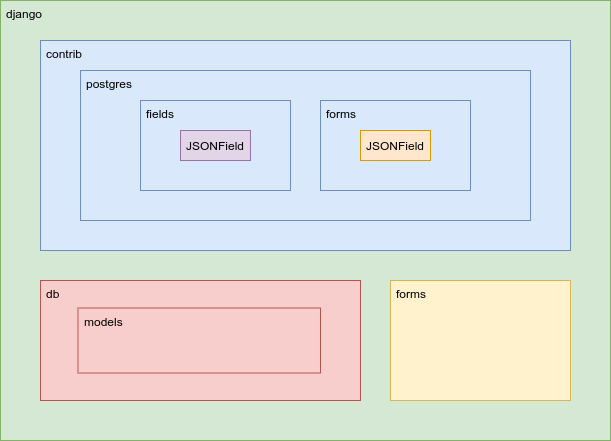
\includegraphics[width=0.85\textwidth]{pics/position1.png}
	\caption{\code{JSONField} classes in Django prior to this research.}
	\label{fig:position1}
\end{figure}

Before this research, the existing \code{JSONField} implementation was included
in the \code{django.contrib.postgres.fields} and
\code{django.contrib.postgres.forms} modules \cite{django30_modeljsonfield,
django30_formjsonfield}. The \code{django.contrib.postgres} module contains
model fields, form fields, and other features that only work with the
PostgreSQL database backend. The locations of the \code{JSONField} classes in
Django prior to this research are illustrated by \autoref{fig:position1} (note
that other Django modules are omitted for brevity).

\begin{figure}
	\centering
    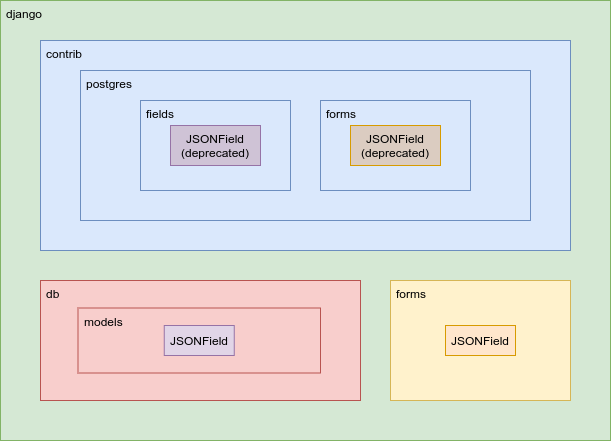
\includegraphics[width=0.85\textwidth]{pics/position2.png}
	\caption{\code{JSONField} classes in Django after this research.}
	\label{fig:position2}
\end{figure}

This research brought \code{JSONField} and other related classes to the
\code{django.db.models} module for the model field and to the
\code{django.forms} module for the form field. Consequently, the previous
implementation was deprecated as of the Django 3.1 release. The previous
implementation would also be removed in the next major release, Django 4.0.

\begin{figure}
	\centering
    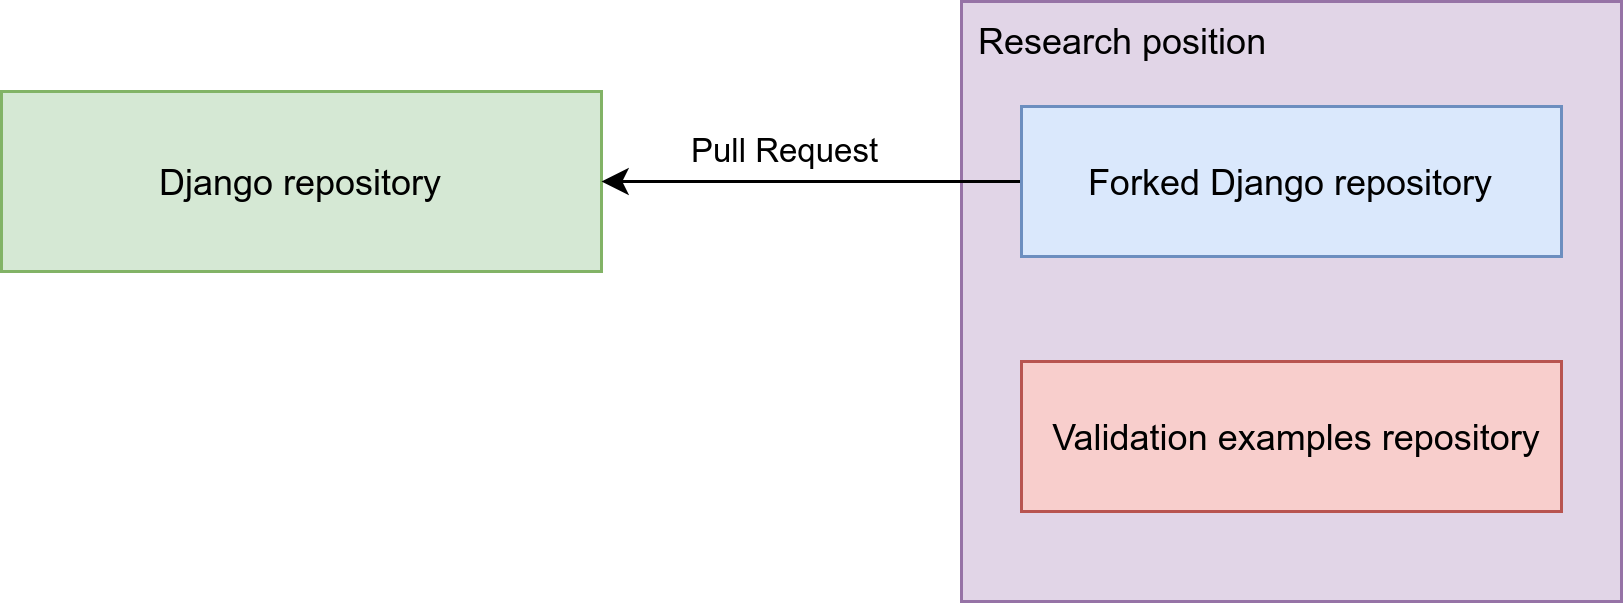
\includegraphics[width=0.85\textwidth]{pics/position3.png}
	\caption{The position of this research.}
	\label{fig:position3}
\end{figure}

This research is mainly split into two parts: the \code{JSONField}
implementation and the analysis demonstrations. The \code{JSONField}
implementation part of the research was done on a Git branch in a GitHub fork
of the Django repository. The branch was submitted as a pull request to the
Django repository to fix ticket \#12990 on the Django issue tracker
\cite{ticket_12990} and was included in the Django 3.1.0 release. The pull
request allowed the Django contributors to review the code and give feedback
on the implementation. The data validation and performance benchmarking
analysis demonstrations were done in a separate repository in the form of
two small Django projects. The position of this research is illustrated by
\autoref{fig:position3}.

\begin{figure}
	\centering
    
\includegraphics[width=0.25\textwidth]{pics/GSoC.png}
	\captionsource{The Google Summer of Code
        logo.}{\url{https://developers.google.com/open-source/gsoc/resources/marketing}}
	\label{fig:gsoc}
\end{figure}

The \code{JSONField} implementation was mostly done as part of the Google
Summer of Code 2019 program. Google Summer of Code (GSoC) is an annual program
held by Google that's focused on introducing students to open-source software
development. In GSoC, students work on a three-month programming project under
the guidance of mentors from an open-source organization. The students are
compensated with a stipend from Google for their work. In turn, the
organizations can identify and bring in new contributors who implement new
features and hopefully continue to contribute to the organizations' projects.

%-----------------------------------------------------------------------------%
\section{Research Steps}
%-----------------------------------------------------------------------------%

The following steps were conducted for the research:

\begin{enumerate}
    \item Literature review \\
    This step focused on reading and understanding how the Django
    object-relational mapping (ORM) tool works, as well as JSON support on the
    database backends supported by Django. During this step, the underlying
    concepts of this research were studied in order to accomplish the research
    objectives.

    \item Experiments \\
    In this step, experiments were done by trying out existing \code{JSONField}
    implementations, which included the PostgreSQL implementation in Django, as
    well as third-party packages on the Python Package Index (PyPI). Some
    experiments were also done by modifying a third-party package to work
    better on different database backends.

    \item Implementation \\
    This step focused on the implementation of the \code{JSONField} model and
    form fields. This was initially done by copying the existing implementation
    from the \code{django.contrib.postgres} module to the
    \code{django.db.models} and \code{django.forms} modules. The tests for the
    existing implementation were also copied. From there, the work was to
    modify the \code{JSONField} implementation so that all tests could pass on
    all available database backends.

    After the \code{JSONField} implementation, this step was continued by
    implementing the data validation example and benchmarking. This included
    the creation of two small Django projects for demonstration purposes.

    \item Results Analysis \\
    In this step, the primary work was to document the different behaviors and
    support of the \code{JSONField} implementation on each database backend.
    This step also included analyzing the data validation and benchmarking
    implementations. For the benchmark, the analysis included comparing the
    performance of \code{JSONField} on all database backends.
\end{enumerate}

%-----------------------------------------------------------------------------%
\section{Report Structure}
%-----------------------------------------------------------------------------%

The structure of this report is as follows:

\begin{itemize}
    \item Chapter 1 \babSatu \\
        This chapter covers the background, problem definition, objectives,
        scope, position, and steps of this research.
    \item Chapter 2 \babDua \\
        This chapter covers the results of the literature review done prior to
        executing the research.
    \item Chapter 3 \babTiga \\
        This chapter covers the design and analysis to prepare for the
        implementation.
    \item Chapter 4 \babEmpat \\
        This chapter covers the \code{JSONField}, the data validation example,
        and the benchmarking implementations.
    \item Chapter 5 \babLima \\
        This chapter covers the analysis of the implementation results. This
        also covers the comparison of the benchmarking results between the
        database backends.
    \item Chapter 6 \kesimpulan \\
        This chapter covers the conclusions of the research and some
        recommendations for further research.
\end{itemize}

\clearchapter
%-----------------------------------------------------------------------------%
\chapter{\babDua}
%-----------------------------------------------------------------------------%

This chapter focuses on building a conceptual framework by reviewing existing
literature and documentation of the underlying concepts of this research.

%-----------------------------------------------------------------------------%
\section{Web Framework}
%-----------------------------------------------------------------------------%

A web framework is a software framework that is designed to support the
development of web applications. It consists of reusable components that solve
common problems in web application development. Most web frameworks provide
safe defaults to prevent security problems in the web application. This helps
programmers build web applications faster and safer. Some web frameworks also
help maintain better application structure by enforcing software design
patterns.

The common components of a web framework are the dispatcher, the decoder, the
generator, and the store \cite{schwarz_webframework}. The dispatcher maps
Uniform Resource Locators (URLs) to application code that is invoked when an
HTTP request is received. The decoder decodes the client request, which allows
the web application to read parameters, headers, and request body data sent as
part of the request. The generator constructs the output that is sent as a
response to the client. The store holds inter-request data, which is usually
stored in a database system.

%-----------------------------------------------------------------------------%
\section{Django}
%-----------------------------------------------------------------------------%

Django is a free and open-source web framework written in Python \cite{django}.
Its overall philosophies are loose coupling, less code, quick development,
don't repeat yourself (DRY), explicit is better than implicit, and consistency
\cite{django:philosophies}. It follows what it calls the model-template-view
architectural pattern, which shares similarities to the model-view-controller
pattern \cite{django:faq}. It consists of an object-relational mapper (ORM)
that handles the interaction with database systems, a template system that
defines how the data looks like to the user, and a view system that defines
which data is presented to the user.

The ORM in Django maps data models to relational database tables. The data
models are represented as Python classes. The model class also has attributes,
called model fields, which represent the columns of the database table. These
model fields define the data types that are used in the database. For example,
the CharField model field uses the VARCHAR data type in the database. In
addition, these model fields also define the behavior of the columns, such as
their NOT NULL and UNIQUE constraints in the database.

Django officially supports five database backends: PostgreSQL, MySQL, MariaDB,
SQLite, and Oracle Database \cite{django:databases}. Each database backend
(other than SQLite) requires a compatible database driver to be installed. The
database backends provided by Django adapt the database drivers so that they
can be used with the ORM. These backends are implemented in the
django.db.backends module.

%-----------------------------------------------------------------------------%
\section{JSON}
%-----------------------------------------------------------------------------%

JavaScript Object Notation (JSON) is a data-interchange format
\cite{ecma:json}. It is designed to be human-readable and easy for machines to
parse and generate. It is based on a subset of the JavaScript standard, but it
is completely language independent. It uses conventions that are similar to
popular programming languages such as C, C++, C\#, Java, JavaScript, Python,
and many others. These properties make JSON a widely-used data-interchange
format, especially in web applications.

JSON is built on two structures: an unordered set of key-value pairs (called
JSON objects) and an ordered list of values (called JSON arrays). The values
can be scalar values such as strings, numbers, booleans, or null. However, they
can also be JSON objects or JSON arrays, which means that they can be nested
to form more complex data structures. An example of a JSON object that contains
a JSON array and other JSON objects can be seen in \autoref{code:json}.

\lstinputlisting[
	language=Python,
	caption=A JSON object,
	label=code:json]{codes/2-json.json}

%-----------------------------------------------------------------------------%
\subsection{Bold, Italic, dan Underline}
%-----------------------------------------------------------------------------%
Hal pertama yang mungkin ditanyakan adalah bagaimana membuat huruf tercetak
tebal, miring, atau memiliki garis bawah. Pada Texmaker, Anda bisa melakukan
hal ini seperti halnya saat mengubah dokumen dengan OO Writer. Namun jika tetap
masih tertarik dengan cara lain, ini dia:

\begin{itemize}
	\item \bo{Bold} \\
	Gunakan perintah \code{\bslash{}textbf$\lbrace\rbrace$} atau
	\code{\bslash{}bo$\lbrace\rbrace$}.
	\item \f{Italic} \\
	Gunakan perintah \code{\bslash{}textit$\lbrace\rbrace$} atau
	\code{\bslash{}f$\lbrace\rbrace$}.
	\item \underline{Underline} \\
	Gunakan perintah \code{\bslash{}underline$\lbrace\rbrace$}.
	\item $\overline{Overline}$ \\
	Gunakan perintah \code{\bslash{}overline}.
	\item $^{superscript}$ \\
	Gunakan perintah \code{\bslash{}$\lbrace\rbrace$}.
	\item $_{subscript}$ \\
	Gunakan perintah \code{\bslash{}\_$\lbrace\rbrace$}.
\end{itemize}

Perintah \code{\bslash{}f} dan \code{\bslash{}bo} hanya dapat digunakan jika
package \code{uithesis} digunakan.


%-----------------------------------------------------------------------------%
\subsection{Memasukan Gambar}
%-----------------------------------------------------------------------------%
Setiap gambar dapat diberikan caption dan diberikan label. Label dapat
digunakan untuk menunjuk gambar tertentu. Jika posisi gambar berubah, maka
nomor gambar juga akan diubah secara otomatis. Begitu juga dengan seluruh
referensi yang menunjuk pada gambar tersebut. Contoh sederhana adalah
\pic~\ref{fig:testGambar}. Silahkan lihat code \latex~dengan nama bab2.tex
untuk melihat kode lengkapnya. Harap diingat bahwa caption untuk gambar selalu
terletak dibawah gambar.

\begin{figure}
	\centering
	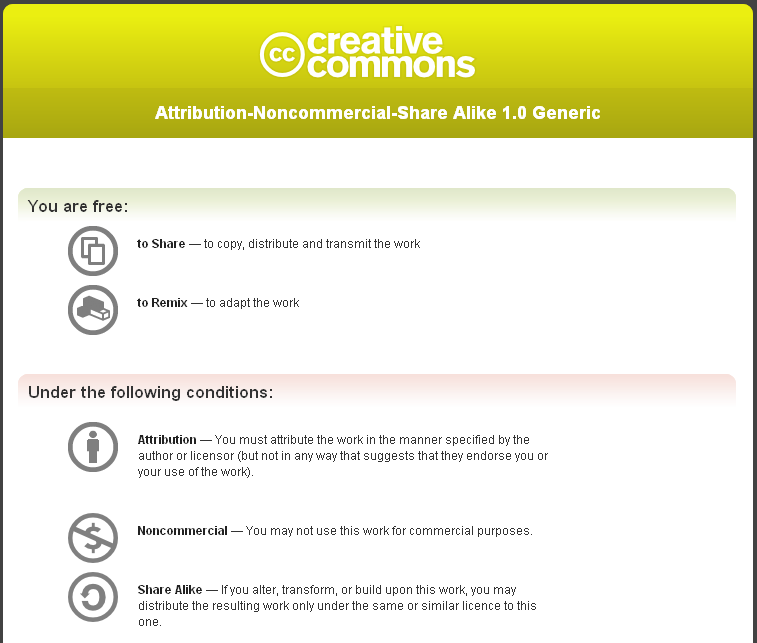
\includegraphics[width=0.50\textwidth]
	{pics/creative_commons.png}
	\caption{\license.}
	\label{fig:testGambar}
\end{figure}


%-----------------------------------------------------------------------------%
\section{Membuat Tabel}
%-----------------------------------------------------------------------------%
Seperti pada gambar, tabel juga dapat diberi label dan caption. Caption pada
tabel terletak pada bagian atas tabel. Contoh tabel sederhana dapat dilihat
pada \tab~\ref{tab:tab1}.

\begin{table}
	\centering
	\caption{Contoh Tabel}
	\label{tab:tab1}
	\begin{tabular}{| l | c r |}
		\hline
		& kol 1 & kol 2 \\
		\hline
		baris 1 & 1 & 2 \\
		baris 2 & 3 & 4 \\
		baris 3 & 5 & 6 \\
		jumlah  & 9 & 12 \\
		\hline
	\end{tabular}
\end{table}

Ada jenis tabel lain yang dapat dibuat dengan \latex~berikut beberapa
diantaranya. Contoh-contoh ini bersumber dari
\url{http://en.wikibooks.org/wiki/LaTeX/Tables}

\begin{table}
	\centering
	\caption{An Example of Rows Spanning Multiple Columns}
	\label{row.spanning}
	\begin{tabular}{|l|l|*{6}{c|}} \hline % create horizontal line
		No & Name & \multicolumn{3}{|c|}{Week 1} & \multicolumn{3}{|c|}{Week 2}
		\\
		\cline{3-8} % create line from 3rd column till 8th column
		& & A & B & C & A & B & C\\
		\hline
		1 & Lala & 1 & 2 & 3 & 4 & 5 & 6\\
		2 & Lili & 1 & 2 & 3 & 4 & 5 & 6\\
		3 & Lulu & 1 & 2 & 3 & 4 & 5 & 6\\
		\hline
	\end{tabular}
\end{table}

\begin{table}
	\centering
	\caption{An Example of Columns Spanning Multiple Rows}
	\label{column.spanning}
	\begin{tabular}{|l|c|l|}
		\hline
		Percobaan & Iterasi & Waktu \\
		\hline
		Pertama & 1 & 0.1 sec \\ \hline
		\multirow{2}{*}{Kedua} & 1 & 0.1 sec \\
		& 3 & 0.15 sec \\
		\hline
		\multirow{3}{*}{Ketiga} & 1 & 0.09 sec \\
		& 2 & 0.16 sec \\
		& 3 & 0.21 sec \\
		\hline
	\end{tabular}
\end{table}

\begin{table}
	\centering
	\caption{An Example of Spanning in Both Directions Simultaneously}
	\label{mix.spanning}
	\begin{tabular}{cc|c|c|c|c|}
		\cline{3-6}
		& & \multicolumn{4}{|c|}{Title} \\ \cline{3-6} & & A & B & C & D \\
		\hline
		\multicolumn{1}{|c|}{\multirow{2}{*}{Type}} & \multicolumn{1}{|c|}{X} &
		1 & 2 & 3 & 4\\ \cline{2-6} \multicolumn{1}{|c|}{}
		& \multicolumn{1}{|c|}{Y} & 0.5 & 1.0 & 1.5 & 2.0\\ \cline{1-6}
		\multicolumn{1}{|c|}{\multirow{2}{*}{Resource}} &
		\multicolumn{1}{|c|}{I} & 10 & 20 & 30 & 40\\ \cline{2-6}
		\multicolumn{1}{|c|}{}                        & \multicolumn{1}{|c|}{J}
		& 5 & 10 & 15 & 20\\ \cline{1-6}
	\end{tabular}
\end{table}


%-----------------------------------------------------------------------------%
\section{Keterkaitan Teori Dengan Penelitian}
%-----------------------------------------------------------------------------%
\todo{Ada baiknya setelah menjelaskan teori-teori, Anda menjelaskan apa kaitan teori tersebut dengan penelitian Anda. Hal ini tentunya membantu pembaca dalam memahami bahwa teori yang Anda paparkan memang penting untuk memahami penelitian Anda nantinya.}

\begin{figure}
	\centering
	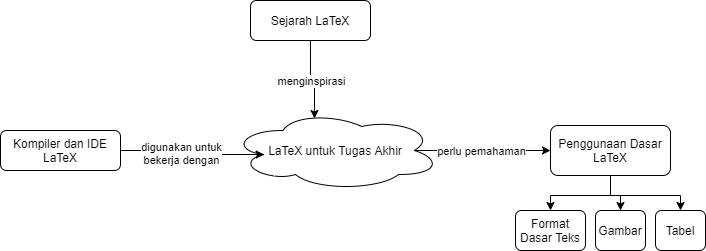
\includegraphics[width=\textwidth]{pics/research_concept_map.png}
	\caption{Keterkaitan konsep hasil studi literatur terhadap penelitian}
	\label{fig:research_concept_map}
\end{figure}

\todo{Jelaskan \pic~\ref{fig:research_concept_map} di sini. Setiap gambar pada
tugas akhir butuh penjelasan. Gambar hadir untuk mempermudah membaca memahami
konteks, tetapi tidak bisa berdiri sendiri tanpa penjelasan. Terkait gambar,
Anda juga bisa mengatur skalanya. Gambar kali ini lebarnya 0,8x dari lebar teks
halaman.}

\clearchapter
%-----------------------------------------------------------------------------%
\chapter{\babTiga}
%-----------------------------------------------------------------------------%

This chapter explains the design and analysis of the \code{JSONField}
implementation, as well as \code{JSONField} data validation examples.

%-----------------------------------------------------------------------------%
\section{\code{JSONField}}
%-----------------------------------------------------------------------------%

There are two kinds of \code{JSONField}: the model field and the form field.
The model field is used as an abstraction of the JSON data in the database,
which lets its users manipulate JSON data in the form of Python objects.
The form field is used for accepting JSON data in forms, such as a Django
\code{ModelForm}. Both fields can be validated using Django's built-in
validation feature with custom-made validator functions.

The model field holds JSON data that can be stored to and retrieved from the
database. In Python, the data is represented in Python's built-in formats:
dictionaries, lists, strings, numbers, booleans, and \code{None}. When saving
the model, Django executes an SQL \code{INSERT} or \code{UPDATE} query to the
database. In order to pass the JSON data in the SQL query, the data has to be
serialized into a JSON-encoded string. When retrieving the model instance,
Django executes an SQL \code{SELECT} query to the database. The data is
retrieved as a JSON-encoded string, which needs to be deserialized, or decoded,
into a Python object.

Python has a built-in \code{json} library that can be used to encode/decode
Python objects into/from JSON-encoded strings \cite{python:json}. The encoding
and decoding functionalities are provided through the \code{json.dumps()} and
\code{json.loads()} functions, respectively, as shown in
\autoref{fig:encodecode}. By default, the \code{json.dumps()} function uses the
\code{json.JSONEncoder} class, while the \code{json.loads()} function uses the
\code{json.JSONDecoder} class. These classes support the Python \code{dict},
\code{list}, \code{str}, \code{int}, \code{float}, \code{True}, \code{False},
and \code{None} data types and objects. To support other data types and
objects, customized \code{json.JSONEncoder} and \code{json.JSONDecoder}
subclasses can be used for the functions by supplying the subclass as the
\code{cls} argument.

\begin{figure}
	\centering
    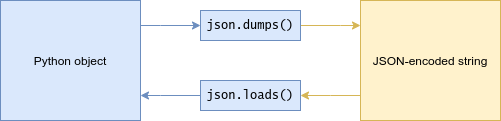
\includegraphics[width=0.66\textwidth]{pics/encodecode.png}
	\caption{The use of the \code{json.dumps()} and \code{json.loads()}
	functions to encode a Python object and decode a JSON-encoded string,
	respectively.}
	\label{fig:encodecode}
\end{figure}

The form field utilizes the \code{json} library for serialization and
deserialization when handling JSON input from the client. If the data being
deserialized is not a valid JSON document, the \code{json.loads()} function
will raise a \code{JSONDecodeError}. This error is used by Django to provide
a basic validation functionality by catching the error and raising a
\code{ValidationError} instead.

\begin{table}
	\centering
	\texttt{
\begin{tabular}{|c|c|c|c|}
\hline
\no{Python}    & \no{JSON} & \no{SQL}            & \no{JSON-encoded string} \\ \hline
'' \no{or} ""  & ""        & ''                  & '""'                     \\ \hline
\{\}           & \{\}      & \no{not applicable} & '\{\}'                   \\ \hline
[]             & []        & \no{not applicable} & '[]'                     \\ \hline
None           & null      & NULL                & 'null'                   \\ \hline
\end{tabular}
}
	\caption{Comparison of empty values and their equivalents in Python, JSON, and SQL.
	The "JSON-encoded string" column shows the Python values after serialization
	with \code{json.dumps()}.}
	\label{table:emptyvalues}
\end{table}

When serializing and deserializing JSON data for the model field, the Python
\code{None} object, the JSON \code{null} value, and the SQL \code{NULL} value
should be taken into consideration. The model field uses JSON-encoded strings
to store JSON values, as there are no SQL equivalents for JSON objects and
arrays. Following the patterns of other values shown in
\autoref{table:emptyvalues}, the \code{None} object should be stored as the
JSON-encoded \code{'null'} string on the database. However, according to the
Python DB-API 2.0 specification (which Django follows), the \code{None} object
is reserved for the SQL \code{NULL} value for both input and output
\cite{db-api2}. Therefore, the model field should skip the serialization and
deserialization for \code{None} (if it's stored as the top-level value) and let
the database driver store it as SQL \code{NULL}.

In order to store and query the JSON \code{null} value as the top-level value
of \code{JSONField}, the \code{Value} class from the \code{django.db.models}
module can be utilized. A \code{Value()} object wraps a literal SQL value to be
used in an SQL expression \cite{django:value}. This literal SQL value is not
processed by Django. In the case of \code{JSONField}, that means the value is
not passed into the \code{json.dumps()} function. Therefore, the JSON
\code{null} value can be stored as a JSON-encoded SQL string literal (i.e.
\code{Value('null')}), which will be stored as \code{'null'} and not
\code{'"null"'} nor \code{NULL}.

\noindent
\begin{minipage}{\linewidth}
\lstinputlisting[language=Python, caption={A \code{Dog} model with a
\code{CharField} for its name and a \code{JSONField} for additional data.},
label=code:dog]{codes/3-dog.py}
\end{minipage}

\noindent
\begin{minipage}{\linewidth}
\lstinputlisting[language=Python, caption={\code{JSONField} behavior with
SQL \code{NULL} and JSON \code{null}.},
label=code:null]{codes/3-null.py}
\end{minipage}

However, when retrieved from the database, both SQL \code{NULL} and
JSON-encoded \code{'null'} are represented in Python with \code{None}. This
happens because Django processes the \code{'null'} value using
\code{json.loads()}, which will return \code{None}. When \code{None} is saved
as a top-level value in the database, it will be saved as SQL \code{NULL}.
Meanwhile, when querying, \code{None} is always interpreted as JSON
\code{null}. To query for SQL \code{NULL}, the \code{isnull} lookup is used.
\autoref{code:null} shows a demonstration of how storing and querying SQL
\code{NULL} and JSON \code{null} work with a \code{JSONField} defined in the
\code{Dog} model shown in \autoref{code:dog}. This behavior may cause confusion
as discussed on the GitHub pull request shown
in \autoref{fig:nulldiscussion}.\footnote{\url{
	https://github.com/django/django/pull/11452\#discussion\_r335375254}}
To avoid this confusion, Django does not recommend working with JSON
\code{null} as the top-level value of \code{JSONField}.

\begin{figure}
	\centering
    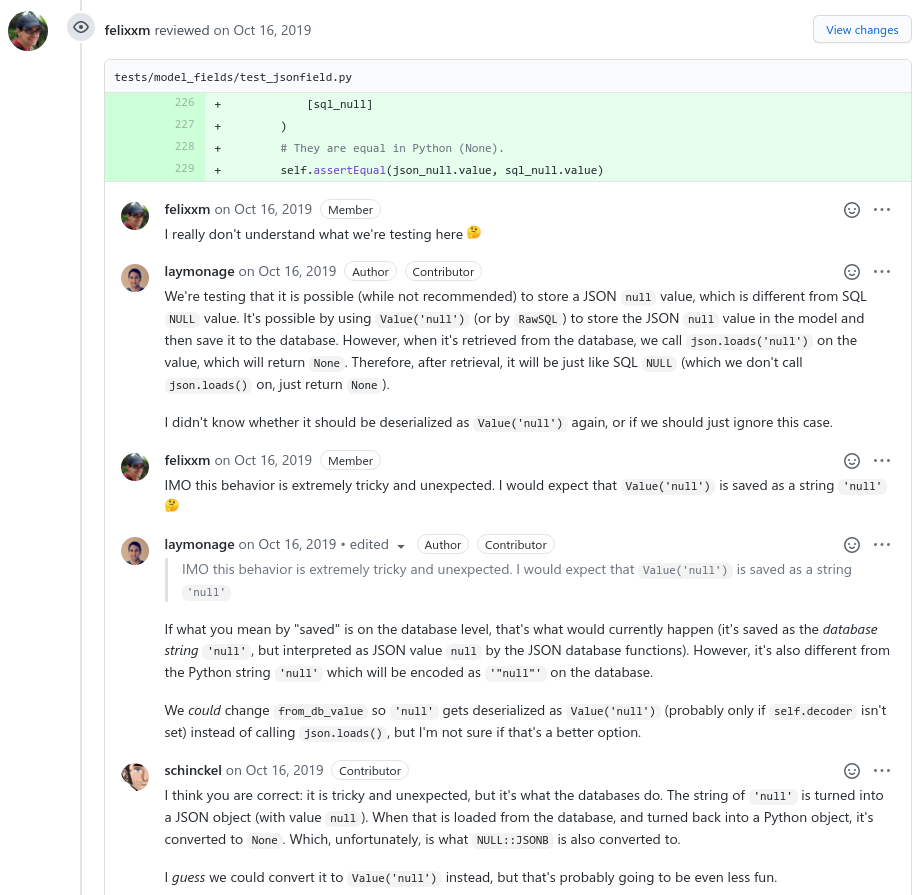
\includegraphics[width=1.0\textwidth]{pics/null_discussion.png}
	\caption{A brief discussion regarding the use of JSON \code{null} as the
	top-level value of a \code{JSONField}.}
	\label{fig:nulldiscussion}
\end{figure}

As with string-based fields such as \code{CharField} and \code{TextField},
Django recommends avoiding the use of SQL \code{NULL} for \code{JSONField}. If
the SQL \code{NULL} is used on a string-based field, it means that there are
two possible values for "no data": \code{NULL} and the empty string
(\code{''}). On \code{JSONField}, it means that there are the empty JSON object
(\code{'\{\}'}), the empty JSON array (\code{'[]'}), the empty JSON string
(\code{'""'}), the JSON \code{null} value (\code{'null'}), and the SQL
\code{NULL}. To avoid redundancy, Django recommends setting \code{null=False}
(to enforce database-level \code{NOT NULL} constraint) and providing a suitable
default for empty values, such as \code{default=dict}.

%-----------------------------------------------------------------------------%
\section{\code{JSONField} Lookups and Transforms}
%-----------------------------------------------------------------------------%

To query JSON data, the previous implementation of \code{JSONField} included
\code{JSONField}-specific lookups and transforms. The lookups and transforms
consisted of containment lookups, key existence lookups, and path transforms.
These lookups and transforms were implemented by using JSON operators that are
only available on PostgreSQL. To implement them on other database systems,
those operators need to be substituted with their JSON function equivalents.

\noindent
\begin{minipage}{\linewidth}
\lstinputlisting[language=Python, caption={A demonstration of how the
\code{contains} and \code{contained\_by} lookups are used.},
label=code:containment]{codes/3-containment.py}
\end{minipage}

The containment lookups consist of the \code{contains} and \code{contained\_by}
lookups. The \code{contains} lookup is overridden on \code{JSONField}.
Normally, it is used to query for strings using a case-sensitive substring
containment test. On \code{JSONField}, it is used to query for JSON data using
a subset containment test. The query will return objects with JSON data that
contains the lookup value as a subset. Meanwhile, the \code{contained\_by}
lookup is the inverse of the \code{contains} lookup, which means that it looks
for objects with JSON data that is contained by the lookup value. The
\code{contains} and \code{contained\_by} lookups are demonstrated in
\autoref{code:containment}.

The containment lookups can be implemented using JSON operators or JSON
functions provided by some of the database systems. On PostgreSQL, the
\code{contains} and \code{contained\_by} lookups can be implemented using the
\code{@>} and \code{<@} operators, respectively. On MariaDB and MySQL, both
lookups can be implemented using the \code{JSON\_CONTAINS} function by
switching the first and second arguments for the \code{contained\_by} lookup.
Unfortunately, SQLite and Oracle Database do not have a similar function, so
these lookups are left unsupported on both databases.

% Key Existence Lookups

% Key, Index, and Path Transforms

\clearchapter
%-----------------------------------------------------------------------------%
\chapter{\babEmpat}
%-----------------------------------------------------------------------------%

This chapter explains the implementation of \verb|JSONField| and
\verb|JSONField|-specific lookups and transforms that can be used on all
database backends supported by Django. The code can be seen in the pull
requests to the Django repository on GitHub
\cite{django:jsonfield-pr, django:contains-pr}.

%-----------------------------------------------------------------------------%
\section{Database Backend Adjustments}
%-----------------------------------------------------------------------------%

Before implementing the \verb|JSONField| class, it is important to remember
that the database systems have different ways of handling JSON data. For
example, each database system uses a different data type to store JSON data. In
addition, the database driver (e.g. Psycopg 2 for PostgreSQL) may automatically
deserialize JSON data into Python objects. When implementing \verb|JSONField|,
these differences need to be taken into account.

Django keeps track of the database systems' differences in the
\verb|django.db.backends| module. Each database system has its own database
backend submodule.\footnote{Except for MariaDB and MySQL, as they can share the
same driver and backend.} The database backends' classes are extended from the
classes in the \verb|django.db.backends.base| submodule. For example, the
\verb|DatabaseFeatures| class stores boolean flags and other feature-related
information as the class' attributes, and the default values for these
attributes are defined in the \verb|BaseDatabaseFeatures| class.

\listing
{Python}
{The new flags for \code{JSONField} in the \code{BaseDatabaseFeatures} class.}
{code:basedbfeatures}
{codes/4-basedbfeatures.py}

To implement the \verb|JSONField| class, three flags are added to the
\verb|BaseDatabaseFeatures| class. The first flag is
\verb|supports_json_field|, which shows whether the database system supports
\verb|JSONField|. The second flag is \verb|supports_primitives_in_json_field|,
which is used to determine whether the database system supports storing JSON
scalar values (strings, numbers, booleans, and \verb|null|) directly in a
\verb|JSONField|. This flag is not used in the \code{JSONField} implementation
itself, but it is used for testing. The third flag is
\verb|has_native_json_field|, which shows whether the database system has a
native JSON data type and the database driver automatically deserializes JSON
data into Python objects. These flags are overridden in each database backend's
\verb|DatabaseFeatures| class as necessary.

\listing
[0 pt]
{Python}
{The \code{DatabaseWrapper} class of the PostgreSQL backend.}
{code:backends-postgresql-1}
{codes/4-backends-postgresql-1.py}

For the PostgreSQL database backend, the \verb|DatabaseWrapper| class is
modified to add support for \verb|JSONField|. The \verb|data_types| property of
the class is updated to map \verb|JSONField| to the \verb|jsonb| data type, as
shown by line 7 of the listing. The \verb|jsonb| data type automatically checks
whether the data is valid according to the JSON syntax, hence there is no need
for a \verb|CHECK| constraint.

\listing
{Python}
{The \code{DatabaseFeatures} class of the PostgreSQL backend.}
{code:backends-postgresql-2}
{codes/4-backends-postgresql-2.py}

Among the new database feature flags, only one flag is overridden for
PostgreSQL. PostgreSQL has a native JSON data type and the driver (Psycopg 2)
automatically deserializes JSON data into Python objects. Thus, the
\verb|has_native_json_field| flag in the \verb|DatabaseFeatures| class of the
backend is set to \verb|True|, as shown by line 4 of
\autoref{code:backends-postgresql-2}. The \verb|supports_json_field| flag is
not overridden because Django supports PostgreSQL 9.5 and higher, while
\code{jsonb} is available as of version 9.4, hence \code{JSONField} is always
supported. The \verb|supports_primitives_in_json_field| flag is also not
overridden, as the value from \verb|BaseDatabaseFeatures| is already correct.

\listing
{Python}
{The \code{DatabaseOperations} class of the PostgreSQL backend.}
{code:backends-postgresql-3}
{codes/4-backends-postgresql-3.py}

To allow a custom decoder for \verb|JSONField| on PostgreSQL, Psycopg 2's
automatic deserialization of JSON data should be disabled. Disabling it can be
done by casting the data to \verb|text| or registering a stub function for
Psycopg 2's \verb|jsonb| converter \cite{psycopg2:json-adaptation}. The casting
option was chosen during this research, as registering a stub function may
break compatibility with the previous implementation that relied on the
automatic deserialization. The casting operation is efficient and does not
involve a copy, hence this decision should not significantly affect the
performance of \code{JSONField} \cite{psycopg2:json-adaptation}. The casting
operation is stored as a method in the \verb|DatabaseOperations| class of the
backend. For PostgreSQL, casting data to \verb|text| can be done using the
\verb|::text| syntax, as shown by line 6 of
\autoref{code:backends-postgresql-3}.

\listing
{Python}
{The \code{DatabaseWrapper} class of the MySQL backend.}
{code:backends-mysql-1}
{codes/4-backends-mysql-1.py}

The MySQL database backend, which is used for MariaDB and MySQL, is modified to
add support for \verb|JSONField|. For this backend, the \verb|DatabaseWrapper|
class is modified by adding a mapping from \verb|JSONField| to the \verb|json|
data type in the \verb|data_types| property, as shown by line 6 of
\autoref{code:backends-mysql-1}. The \verb|data_type_check_constraints|
property method is also modified to add the \verb|JSON_VALID()| function as a
\verb|CHECK| constraint for MariaDB prior to version 10.4.3, as shown by lines
15 and 16 of the listing. Later versions of MariaDB have the \verb|CHECK|
constraint automatically enabled when using the \verb|JSON| data type alias,
while MySQL automatically validates the JSON syntax when using the \verb|JSON|
data type. Therefore, there is no need to modify
\verb|data_type_check_constraints| for these systems.

\listing
{Python}
{The \code{DatabaseFeatures} class of the MySQL backend.}
{code:backends-mysql-2}
{codes/4-backends-mysql-2.py}

For MariaDB and MySQL, the \verb|DatabaseFeatures| class is modified by turning
\verb|supports_json_field| into a cached property method. The method returns
\verb|True| for MariaDB version 10.2.7 or higher and MySQL version 5.7.8 or
higher (and \verb|False| otherwise), as shown by lines 4 to 8 of
\autoref{code:backends-mysql-2}. The other flags
(\verb|supports_primitives_in_json_field| and \verb|has_native_json_field|)
use the values from \verb|BaseDatabaseFeatures| as they are already correct.

\listing
{Python}
{The \code{DatabaseWrapper} class of the SQLite backend.}
{code:backends-sqlite3-1}
{codes/4-backends-sqlite3-1.py}

For the SQLite database backend, the \verb|DatabaseWrapper| class is modified
to add the mapping from \verb|JSONField| to \verb|text| in the
\verb|data_types| property, as shown by line 7 of
\autoref{code:backends-sqlite3-1}. It is also modified to apply the
\verb|JSON_VALID()| SQL \verb|CHECK| constraint to the database column. As the
function returns \verb|0| (false) for SQL \verb|NULL| values, an
\verb|OR "%(column)s" IS NULL| clause is added to support storing SQL
\verb|NULL| values, as shown by line 12 of the listing.

\listing
{Python}
{The \code{DatabaseFeatures} class of the SQLite backend.}
{code:backends-sqlite3-2}
{codes/4-backends-sqlite3-2.py}

Meanwhile, \verb|DatabaseFeatures| class is modified to check for JSON support
on SQLite. The \verb|supports_json_field| flag is turned into a cached property
method and the value is determined by trying to execute a \verb|SELECT| query
with the \verb|JSON()| function included in the JSON1 extension, as shown by
lines 4 to 8 of \autoref{code:backends-sqlite3-2}. If the query does not throw
an exception, that means the JSON1 extension is enabled and the flag is set to
\verb|True| (and \verb|False| otherwise), as shown by lines 9 to 11 of the
listing. The support check is done this way because SQLite does not provide a
direct way to check whether the JSON1 extension is loaded. The other
flags (\verb|supports_primitives_in_json_field| and
\verb|has_native_json_field|) are derived from \verb|BaseDatabaseFeatures|, as
the values are already correct.

\listing
{Python}
{The \code{DatabaseWrapper} class of the Oracle Database backend.}
{code:backends-oracle-1}
{codes/4-backends-oracle-1.py}

For the Oracle Database backend, the \verb|DatabaseWrapper| class is modified
to add the data type mapping and \verb|CHECK| constraint. The \verb|data_types|
property is updated to map \verb|JSONField| to \verb|NCLOB|, as shown by line 7
of \autoref{code:backends-oracle-1}. The \code{NCLOB} data type is chosen to
allow data larger than 32,767 bytes and to have Unicode support
\cite{oracle:overview-json, oracle:database-concepts}. The
\verb|data_type_check_constraints| property is also updated to apply the
\verb|IS JSON| constraint for \verb|JSONField|, as shown by line 12 of the
listing.

\listing
{Python}
{The \code{DatabaseOperations} class of the Oracle Database backend.}
{code:backends-oracle-2}
{codes/4-backends-oracle-2.py}

The cx\_Oracle database driver returns \verb|CLOB| and \verb|BLOB| values from
the database as \verb|LOB| objects in Python \cite{cxoracle:lob}. Meanwhile,
the \verb|LOB| objects need to be converted to Python strings in order to
perform deserialization. To do this, the \verb|get_db_converters()| method in
the \verb|DatabaseOperations| class is overridden so that \verb|JSONField| uses
the \verb|convert_textfield_value| converter, as shown by lines 7 and 8 of
\autoref{code:backends-oracle-2}. The \code{TextField} model field also uses
the \code{NCLOB} data type on Oracle Database and, as a result, the converter
can be reused for \code{JSONField}.

\listing
{Python}
{The \code{DatabaseFeatures} class of the Oracle Database backend.}
{code:backends-oracle-3}
{codes/4-backends-oracle-3.py}

For Oracle Database, only the \verb|supports_primitives_in_json_field| flag is
overridden in the \verb|DatabaseFeatures| class. The flag is overridden to
\verb|False|, as shown by line 4 of \autoref{code:backends-oracle-2}. This flag
reflects the behavior of Oracle Database that only allows storing JSON objects
and arrays in a column with the \verb|IS JSON| constraint enabled. The
\verb|supports_json_field| flag is not overridden because Oracle Database
introduced JSON support in version 12.1.0.2 and Django supports Oracle Database
version 12.2 and higher, hence \code{JSONField} is always supported. The
\verb|has_native_json_field| flag is derived from \verb|BaseDatabaseFeatures|
because the value is already correct.

All database backends have now been adjusted with the necessary changes. The
changes were mostly made for mapping \verb|JSONField| to the correct data type
on the database, as well as the \verb|CHECK| constraints to ensure that the
data is valid JSON. With these changes in place, the \verb|JSONField| class can
now be implemented.

%-----------------------------------------------------------------------------%
\section{\code{JSONField}}
%-----------------------------------------------------------------------------%

In the Django codebase, model fields are defined in the
\verb|django.db.models.fields| module as subclasses of \verb|Field|, but they
can be imported from the \verb|django.db.models| module for convenience. Model
fields that are relatively simple are implemented in the \verb|__init__.py|
file of the module. For model fields that require more complex implementation
(e.g. file fields and relational fields), they are defined in their own files
in the \verb|fields| directory. Due to the complexity of \verb|JSONField| and
its extended querying capabilities, the implementation is defined in the
\verb|json.py| file in the \verb|fields| directory.

\listing
{Python}
{The \code{deconstruct()} method of \code{Field}.}
{code:field-deconstruct}
{codes/4-field-deconstruct.py}

Model fields have a \verb|deconstruct| method that defines how the field can be
reconstructed from a database migration. The method returns a 4-tuple that
consists of: the name of the field on the model, the import path of the field,
a list of positional arguments, and a dictionary of keyword arguments
\cite{django:model_fields}. By convention, model fields that are defined in
their own files like \verb|JSONField| should still be imported from
\verb|django.db.models|. Thus, the \verb|deconstruct()| method of the
\verb|Field| class is modified to shorten the path for \verb|JSONField|'s
module, as shown by lines 15 to 17 of \autoref{code:field-deconstruct}.

\listing
{Python}
{The \code{check()} method of \code{JSONField} model field.}
{code:jsonfield-check}
{codes/4-jsonfield-check.py}

The \verb|JSONField| class implements some checks to make sure that it is used
correctly. In addition to the checks included from the \verb|Field| class,
\verb|JSONField| also extends the \verb|CheckFieldDefaultMixin| class, as shown
by line 1 of \autoref{code:jsonfield-check}. The mixin\footnote{A mixin is a
class that defines methods to be used by other classes through inheritance.}
adds a check to ensure that any default value set for the field should be a
callable instead of an instance, so that it is not shared between all instances
of the field. The \verb|JSONField| class also overrides the \verb|check()|
method to include the \verb|_check_supported()| method in the checking process,
as shown by lines 4 to 8 of the listing.

\listing
{Python}
{The \code{\_check\_supported()} method of \code{JSONField} model field.}
{code:jsonfield-checksupported}
{codes/4-jsonfield-checksupported.py}

The \verb|_check_supported()| method checks all of the connected databases for
\verb|JSONField| support. If migrations for the model (that the field is
attached to) are not allowed on the database by the database router, then the
database is skipped from the check, as shown by lines 4 and 5 of
\autoref{code:jsonfield-checksupported}. Otherwise, the
\verb|supports_json_field| feature flag is checked. Lines 7 to 17 show that if
the flag's value is \verb|False| and the model is not explicitly defined to
require the feature flag, then a system error is added to the lists of errors
to be returned by the \verb|check| method and shown to the programmer.

\listing
{Python}
{The \code{get\_internal\_type()} method of \code{JSONField} model field.}
{code:jsonfield-getinternaltype}
{codes/4-jsonfield-getinternaltype.py}

To determine the key that is used to get the data type and \verb|CHECK|
constraints from the database backends, the \verb|get_internal_type()| method
is used. By default, the method returns the name of the class (using
\verb|self.__class__.__name__|), which means that an override is not necessary.
However, other model fields override the method to explicitly return the name
of the class, so that other classes may extend the model fields without having
to override the \verb|get_internal_type()| method unless it is needed. Thus,
the \verb|get_internal_type()| method is overridden to explicitly return the
string \verb|'JSONField'|, as shown by line 2 of
\autoref{code:jsonfield-getinternaltype}.

\listing
{Python}
{The \code{get\_prep\_value()} method of \code{JSONField} model field.}
{code:jsonfield-ser}
{codes/4-jsonfield-ser.py}

In the previous chapter, \verb|JSONField| is designed to serialize Python
objects into JSON-encoded strings by utilizing the built-in \verb|json| library
in Python. The serialization process is needed in order to store Python objects
as JSON in the database. To convert Python objects to query values, the
\verb|get_prep_value()| method should be overridden. The serialization is shown
by line 4 of \autoref{code:jsonfield-ser}, where the Python object is passed
to the \verb|json.dumps()| function, which also accepts an optional encoder
class as the \verb|cls| argument. Lines 2 and 3 of the listing show that the
\verb|None| value should not be serialized, because it is reserved for SQL
\verb|NULL| as previously explained.

In addition to the serialization needed to store a Python object inside
\verb|JSONField| to the database, Django also has a serialization framework
that can be used for model objects. The framework can be used to dump model
objects into XML, JSON, and YAML files. The framework serializes model objects
by calling the \verb|value_to_string()| method of their fields.

\listing
{Python}
{The \code{value\_to\_string()} method of \code{JSONField} model field.}
{code:jsonfield-valuetostring}
{codes/4-jsonfield-valuetostring.py}

Normally, the \verb|value_to_string()| method returns a string that is ready to
be used by the serializer. However, \verb|JSONField| represents JSON data in
its Python built-in format that can be serialized by the built-in serializers.
Therefore, the method should just return the Python object as-is and let the
serializers handle the serialization process. To achieve this, the
\verb|value_to_string()| method is overridden to just return the field's value.
To get the field's value prior to serialization, the \verb|value_from_object()|
method is used, as shown by line 2 of \autoref{code:jsonfield-valuetostring}.

\listing
{Python}
{The \code{from\_db\_value()} method of \code{JSONField} model field.}
{code:jsonfield-des}
{codes/4-jsonfield-des.py}

\verb|JSONField| is also designed to deserialize JSON-encoded strings to Python
objects in order to load the JSON data from the database. To convert database
values to Python objects, the \verb|from_db_value()| method can be overridden.
On some database systems that have a native JSON data type, the database driver
may already deserialize the value before Django receives it.\footnote{Only
PostgreSQL's Psycopg 2 driver does this at the time of writing, but this may
change in the future.} Lines 4 and 5 of \autoref{code:jsonfield-des} show that
the value is returned as-is, unless a custom decoder is used. In other cases,
the deserialization process is shown by line 7 of the listing, where
the database value is passed to the \verb|json.loads()| function, which also
accepts an optional decoder class as the \verb|cls| argument. Similar to
\verb|get_prep_value()|, the \verb|None| value is reserved for the SQL
\verb|NULL| value, as shown by lines 2 and 3 of the listing.

When extracting JSON string values, the database systems return them as
deserialized values (i.e. without JSON double quotes). Passing deserialized
strings to \verb|json.loads()| may cause \verb|json.JSONDecodeError| to be
raised. Therefore, as shown by lines 6 to 9 of \autoref{code:jsonfield-des},
the \verb|json.loads()| call is put inside a \verb|try ... except| block and
the value is directly returned if \verb|json.JSONDecodeError| is raised.

\listing
{Python}
{The \code{select\_format()} method of \code{JSONField} model field.}
{code:jsonfield-selectformat}
{codes/4-jsonfield-selectformat.py}

To cast JSON data to \verb|text| on the database level, the
\verb|select_format()| method is overridden in the \verb|JSONField| class. The
method determines the format of the \verb|SELECT| clause of the SQL query. The
casting operation is needed in order to enable the use of a custom decoder with
a database system that automatically deserializes JSON data into Python
objects. Thus, the casting operation is performed only if a custom decoder is
used with a database backend that has the \verb|has_native_json_field| feature
flag set to \verb|True|, as shown by lines 2 to 6 of
\autoref{code:jsonfield-selectformat}.

\listing
{Python}
{The \code{\_\_init\_\_()} method (constructor) of \code{JSONField}
model field.}
{code:jsonfield-init}
{codes/4-jsonfield-init.py}

The custom encoder and decoder are stored as instance attributes of the field,
as shown by lines 13 and 14 of \autoref{code:jsonfield-init}. It is important
to note that the encoder and decoder are subclasses of \verb|json.JSONEncoder|
and \verb|json.JSONDecoder|, rather than instances of those classes. In Python,
a class is a callable that returns an instance of the class and, as a result,
the encoder and decoder have to be callables. To enforce this requirement, the
\verb|JSONField| constructor checks whether the encoder and decoder are
callables and raises descriptive error messages if they are not, as shown by
lines 5 to 12 of the listing.

\listing
{Python}
{The \code{deconstruct()} method of \code{JSONField} model field.}
{code:jsonfield-dec}
{codes/4-jsonfield-dec.py}

As the \verb|JSONField| constructor has been modified to add support for custom
encoder and decoder, the \verb|deconstruct()| method needs to be overridden so
that the encoder and decoder are preserved in database migrations. The encoder
and decoder are defined as keyword arguments of the constructor. Therefore, the
\verb|deconstruct()| method is overridden to add the encoder and decoder
classes (if they are set, i.e. not \verb|None|) to the keyword arguments
dictionary, as shown by lines 3 to 6 of \autoref{code:jsonfield-dec}.

\listing
{Python}
{The \code{\_\_init\_\_()} method (constructor) of \code{JSONField} form field.}
{code:formfield-init}
{codes/4-formfield-init.py}

The \verb|JSONField| form field has also been updated to support custom encoder
and decoder. As with the model field, the encoder and decoder classes are
stored as instance attributes of the form field, as shown by lines 8 and 9 of
\autoref{code:formfield-init}. The encoder and decoder classes are used in
\verb|json.dumps()| and \verb|json.loads()| calls throughout the form field,
respectively.

\listing
{Python}
{The \code{prepare\_value()} and \code{has\_changed()} methods of
\code{JSONField} form field.}
{code:formfield-dumps}
{codes/4-formfield-dumps.py}

To utilize a custom encoder, some of the \verb|JSONField| form field methods
had to be updated. Line 4 of \autoref{code:formfield-dumps} shows the encoder
class used in the \verb|json.dumps()| call inside the \verb|prepare_value()|
method, which is used to prepare the value before it is shown to the user (e.g.
in an HTML form). Lines 12 and 13 show the encoder class used in the
\verb|json.dumps()| calls inside the \verb|has_changed()| method, which is used
to check whether the value inside the form field has changed.

\listing
{Python}
{The \code{to\_python()} and \code{bound\_data()} methods of \code{JSONField}
form field.}
{code:formfield-loads}
{codes/4-formfield-loads.py}

Some of the \verb|JSONField| form field methods also had to be updated to
support the use of a custom decoder. Line 4 of \autoref{code:formfield-loads}
shows the decoder class used in the \verb|json.loads()| call inside the
\verb|to_python()| method, which is used in the form field validation process.
If the value cannot be deserialized with the decoder, a \verb|ValidationError|
is raised, as shown by lines 5 to 10. Line 16 shows the decoder class used in
the \verb|json.loads()| call inside the \verb|bound_data()| method, which is
used to load the input data to the form field.

The form field only handles user input and does not interact with the database
directly. Thus, it is already possible to use the \verb|JSONField| form field
with any database backend. As a result, the form field is now moved from the
\verb|django.contrib.postgres.forms| module to the \verb|django.forms| module.

\listing
{Python}
{The \code{formfield()} method of \code{JSONField} model field.}
{code:jsonfield-form}
{codes/4-jsonfield-form.py}

When model fields are included in a \verb|ModelForm|, Django automatically
generate form fields for them \cite{django:modelform}. The form fields are
generated by calling the \verb|formfield()| method of the model fields. In
order to use the encoder and decoder from the \verb|JSONField| model field in
the \verb|JSONField| form field, they need to be passed as keyword arguments,
as shown by lines 4 and 5 of \autoref{code:jsonfield-form}.

\listing
{Python}
{The \code{validate()} method of \code{JSONField} model field.}
{code:jsonfield-validate}
{codes/4-jsonfield-validate.py}

Model fields can define a built-in validation mechanism in the
\verb|validate()| method. The method is called by the field's \verb|clean()|
method as part of the model validation process of a \verb|ModelForm|. For
\verb|JSONField|, the \verb|validate()| method is overridden to provide a
basic validation mechanism by trying to serialize the field's value with the
given encoder, as shown by lines 3 and 4 of \autoref{code:jsonfield-validate}.
Lines 5 to 10 of the listing show that if the serialization fails, then a
\verb|ValidationError| is raised.

Now that the \verb|JSONField| class has been implemented, it is possible to
store and load JSON data to and from the database. As explained in the previous
chapter, there are also lookups and transforms that are specific for
\verb|JSONField|. The lookups and transforms extend the querying capabilities
for \verb|JSONField| by utilizing the functions and operators available on the
database systems. The implementation of the lookups and transforms will be
explained in the next section.

%-----------------------------------------------------------------------------%
\section{\code{JSONField} Lookups and Transforms}
%-----------------------------------------------------------------------------%

Lookups and transforms are part of Django's query expressions API. The API
consists of classes which instances can be compiled by Django's
\verb|SQLCompiler| objects. An \verb|SQLCompiler| object translates a query
expression by calling its \verb|as_vendorname()|\footnote{The \code{vendorname}
is the value of the \code{vendor} attribute in the \code{DatabaseWrapper} class
of the database backend, i.e. \code{postgresql}, \code{mysql}, \code{sqlite},
and \code{oracle}.} method (for vendor-specific implementation) if it exists,
and falls back to the \verb|as_sql()| method otherwise.

The lookups and transforms in this research are specific to \verb|JSONField|.
Normally, lookups and transforms are implemented in the
\verb|django.db.models.lookups| module. In the module, lookups are implemented
as subclasses of the \verb|Lookup| class, while transforms are implemented as
subclasses of the \verb|Transform| class. However, as the lookups and
transforms in this research are specific to \verb|JSONField|, they are
implemented as part of the \verb|django.db.models.fields.json| module.

The lookups that can be used on \verb|JSONField| are the
\verb|JSONField|-specific lookups and some of the built-in lookups. The
\verb|JSONField|-specific lookups are the containment lookups (\verb|contains|
and \verb|contained_by|), as well as the key existence lookups (\verb|has_key|,
\verb|has_keys|, and \verb|has_any_keys|). In addition to the
\verb|JSONField|-specific lookups, some of the built-in lookups (e.g.
\verb|exact|, \verb|isnull|, etc.) need to be modified so that they can be used
on \verb|JSONField|.

The \verb|JSONField| transforms are the key, index, and path transforms that
extract the value of JSON data at a given path. The index transform is just a
special case of the key transform where the key is an integer. Meanwhile, the
path transform can be viewed as a chain of key transforms. Therefore, the
transforms were unified as \verb|KeyTransform| in the existing implementation.

The value extracted by the transforms can be chained with some of the built-in
lookups and the \verb|JSONField|-specific lookups. The value returned by the
transforms may have different data types. As a result, some of the lookups also
need to be modified when they are used on a \verb|KeyTransform|.

The lookups can be used directly on a \verb|JSONField| or on
\verb|KeyTransform|s applied to the field. When some of the lookups are used on
the transforms, they are implemented differently. Thus, before going in-depth
with the lookups implementation, it is better to go through the transforms
first.

\subsection{\code{JSONField} Transforms}

\listing
{Python}
{Parts of the \code{KeyTransform} class.}
{code:keytransform-1}
{codes/4-keytransform-1.py}

The key, index, and path
transforms are unified as the \verb|KeyTransform| class, which can be used to
extract the value of a \verb|JSONField| at a given path. The class includes the
{PostgreSQL} operators for extracting JSON values as shown by lines 2 and 3
of \autoref{code:keytransform-1}. Line 7 shows that the key name is normalized
as a string on initialization.

\listing
{Python}
{The \code{preprocess\_lhs()} method of the \code{KeyTransform} class.}
{code:keytransform-2}
{codes/4-keytransform-2.py}

To process a chain of \verb|KeyTransform|s that make up a path transform, the
\verb|preprocess_lhs()| method is created. Lines 4 to 8 of
\autoref{code:keytransform-2} show how the method separates the chain of
\verb|KeyTransform|s from the previous \verb|lhs|. The separation is done by
traversing the \verb|lhs| attribute of the \verb|KeyTransforms| until the
\verb|lhs| is not a \verb|KeyTransform|. While traversing, the key names that
construct the path are saved into a list. The method then compiles the original
\verb|lhs| and its parameters, and return them along with the list of key
names, as shown by lines 9 and 12. Lines 10 and 11 show that on Oracle
Database, any \verb|%| character in the key name is replaced by
\verb|%%| to escape string formatting (this will be explained later). In
addition, the method also has an \verb|lhs_only| parameter for optimization by
not saving and returning the key names if they are not needed, as shown by
lines 1, 2, 6, and 12.

\listing
{Python}
{The \code{as\_postgresql()} method of the \code{KeyTransform} class.}
{code:keytransform-3}
{codes/4-keytransform-3.py}

To compile a \verb|KeyTransform| into an SQL query expression, the
\verb|as_vendor()| method is used, e.g. \verb|as_postgresql()| for the
PostgreSQL backend. The method uses the \verb|preprocess_lhs()| method
described previously, as shown by line 2 of \autoref{code:keytransform-3}. If
there are multiple \verb|KeyTransform|s, the \verb|postgres_nested_operator|
(\verb|#>|) is used, as shown by lines 3 to 7 of the listing. Otherwise, the
\verb|postgres_operator| (\verb|->|) is used, as shown by lines 12 to 15. For
consistency, if there is only one \verb|KeyTransform| and the key is an
integer, it is assumed to be an array index by converting it to the \verb|int|
data type, as shown by line 9. The conversion is not needed for the nested
operator because for this operator, PostgreSQL automatically interprets integer
key names as array indices.

\listing
{Python}
{The \code{as\_sql()} method of the existing PostgreSQL-only \code{KeyTransform} class.}
{code:keytransform-0}
{codes/4-keytransform-0.py}

During this research, a security vulnerability was found in the existing
PostgreSQL-only implementation of \verb|KeyTransform|. Previously, the SQL
query expression was implemented in the \verb|as_sql()| method because it is
assumed that \verb|KeyTransform| is only used on PostgreSQL (as part of the
\verb|django.contrib.postgres| module). In the method, when there is only one
\verb|KeyTransform|, the key name is directly inserted into the string, rather
than passing it in the SQL parameters, as shown by lines 6, 8, and 9 of
\autoref{code:keytransform-0}. In addition, the key name is also not properly
quoted using \verb|json.dumps()|.

The approach in the existing implementation opened up a way for executing an
SQL injection by using a specially crafted string as the key name. The key name
is usually passed as a keyword argument in Python, which means that the string
can only contain alphanumeric characters and underscores. However, keyword
arguments can also be specified using a dictionary in Python, which allows any
string as a key name.

Using a malicious string as a key name in a dictionary that is passed as keyword
arguments, a user can execute an SQL injection. This vulnerability was reported
via email to the Django security team\footnote{Security issues in Django should
be reported to
\href{mailto:security@djangoproject.com}{security@djangoproject.com}, not the
public issue tracker.} and it was classified as CVE-2019-14234 \cite{cve} with
critical severity. To fix the vulnerability, a patch was issued for the Django
1.11, 2.1, and 2.2 releases \cite{django:securityrelease}. The implementation
of \verb|as_postgresql()| in this research has incorporated the patch, as shown
by lines 8 to 15 of \autoref{code:keytransform-3}.

\listing
{Python}
{The \code{compile\_json\_path()} function.}
{code:compilejsonpath}
{codes/4-compilejsonpath.py}

On other database systems, the JSON extraction functions use the JSONPath
notation to specify the path to be extracted. For reusability, the
\verb|compile_json_path()| function is created to convert a list of key names
into its JSONPath representation. The function works by iterating through the
list of key names and keeping a list of strings that make up the JSONPath. If
the key name is an integer, the string \verb|'[num]'| (where \verb|num| is the
integer) is appended to the list, as shown by lines 4, 5, 9, and 10 of
\autoref{code:compilejsonpath}. Otherwise, the key name is enclosed in double
quotes (so that it may contain spaces) by passing it through
\verb|json.dumps()|, as shown by lines 6 to 8. Additionally, the method also
has a \verb|include_root| parameter to control whether the resulting path
should include the root notation (\verb|$|), as shown by lines 1 and 2.
Finally, the list of strings is concatenated by joining the strings with an
empty string, as shown by line 11.

\listing
{Python}
{The \code{as\_mysql()} and \code{as\_sqlite()} methods of the \code{KeyTransform} class.}
{code:keytransform-4}
{codes/4-keytransform-4.py}

The \verb|as_vendor()| methods for MariaDB, MySQL, and SQLite are similar. The
methods utilize the \verb|preprocess_lhs()| method and
\verb|compile_json_path()| to construct the JSONPath notation of the key
transforms, as shown by lines 2, 3, 7, and 8 of \autoref{code:keytransform-4}.
To extract the value, the \verb|JSON_EXTRACT()| function is used, with
\verb|lhs| as the first argument and the JSONPath as the second argument, as
shown by lines 4 and 9.

\listing
{Python}
{The \code{as\_oracle()} method of the \code{KeyTransform} class.}
{code:keytransform-5}
{codes/4-keytransform-5.py}

Meanwhile, the \verb|as_oracle()| method needs some adjustments to work with
the behavior of Oracle Database. The method still uses the
\verb|preprocess_lhs()| method and \verb|compile_json_path()| function, as
shown by lines 2 and 3 of \autoref{code:keytransform-5}. However, to extract
the value, the \verb|JSON_QUERY()| and \verb|JSON_VALUE()| functions are
combined using the \verb|COALESCE()| function. This approach is needed as there
is no way to tell whether the value at the given path is a JSON object/array or
a scalar value. In addition, the path argument is added directly to the SQL
string, as shown by lines 5 and 6, because path expressions cannot be passed as
bind variables on Oracle Database \cite{oracle:jsonpath}.

\listing
{Python}
{Parts of the \code{Cast} class.}
{code:cast}
{codes/4-cast.py}

The JSON extraction functions are also useful for casting other fields to
\verb|JSONField| if the database system does not have a true data type for
JSON. To cast from one model field to another, Django provides the \verb|Cast|
class that can be used to perform casting on the database level. To support
casting to \verb|JSONField| on databases without a true data type for JSON, the
\verb|as_vendor()| methods of the \verb|Cast| class is overridden. The
\verb|JSON_EXTRACT()| function is used on MariaDB to force data to be
recognized as JSON, as shown by lines 6 to 8 of \autoref{code:cast}. Lines 14
to 16 show that on Oracle Database, the \verb|JSON_QUERY()| function is used.
For SQLite, using the \verb|JSON_EXTRACT()| function is not necessary as the
database can handle JSON data in its string form correctly.

\listing
{Python}
{The \code{KeyTextTransform} class.}
{code:keytexttransform}
{codes/4-keytexttransform.py}

Aside from \verb|KeyTransform|, the \verb|KeyTextTransform| class is also
implemented. The \verb|KeyTransform| class extracts JSON values with the
\verb|jsonb| data type on PostgreSQL. Meanwhile, some built-in lookups expect
the \verb|lhs| to be \verb|text|. Rather than casting the value to \verb|text|,
the \verb|KeyTextTransform| class works by using the \verb|->>| and \verb|#>>|
operators instead of the \verb|->| and \verb|#>| operators, as shown by lines 2
and 3 of \autoref{code:keytexttransform}. The \verb|as_vendor()| methods do not
need to be overridden for other database backends, because they already extract
JSON string values as \verb|text|.

\listing
{Python}
{The \code{KeyTransformFactory} class.}
{code:keytransformfactory}
{codes/4-keytransformfactory.py}

In order to use the transforms, a factory class (\verb|KeyTransformFactory|)
needs to be implemented. The key name of a \verb|KeyTransform| can be any
string as long as it doesn't clash with a registered lookup or transform.
Normally, transforms already have a predefined name for them, hence their
\verb|__init__()| method does not have a parameter for defining the name. As
the key name of a \verb|KeyTransform| is defined dynamically, a factory class
is needed in order to encapsulate the key name information, as shown by line 4
of \autoref{code:keytransformfactory}. The key name will be passed as a
predefined argument when instantiating a \verb|KeyTransform| by calling the
factory object, as shown by lines 6 and 7 of the listing.

\listing
{Python}
{The \code{get\_transform()} method of the \code{JSONField} model field.}
{code:gettransform}
{codes/4-gettransform.py}

The factory instance is then registered to \verb|JSONField| by overriding the
\verb|get_transform()| method of \verb|JSONField| shown by
\autoref{code:gettransform}. The method works by trying to look recursively on
all parent classes for a registered transform with the given name and return it
if found, as shown by lines 2 to 4 of \autoref{code:gettransform}. If the
transform is not found, the method returns a \verb|KeyTransformFactory|
instance with the transform name as the key name, as shown by line 5 of the
listing.

As the transforms have been implemented, the lookups can now be implemented as
well. The lookups consist of the \verb|JSONField|-specific lookups and the
built-in lookups. The \verb|JSONField|-specific lookups are containment lookups
(\verb|contains| and \verb|contained_by|) and key existence lookups
(\verb|has_key|, \verb|has_keys|, and \verb|has_any_keys|). Meanwhile, the
built-in lookups are \verb|exact|, \verb|iexact|, \verb|isnull|,
\verb|icontains|, \verb|startswith|, \verb|istartswith|, \verb|endswith|,
\verb|iendswith|, \verb|regex|, \verb|iregex|, \verb|lt|, \verb|lte|,
\verb|gt|, and \verb|gte|.

\subsection{\code{JSONField} Lookups}

\listing
{Python}
{The \code{PostgresOperatorLookup} class.}
{code:pgop-lookup}
{codes/4-pgop-lookup.py}

In the existing PostgreSQL-only implementation, \verb|JSONField| lookups were
implemented by extending the \verb|PostgresSimpleLookup| class. The class was
an abstraction for the \verb|<lhs> <operator> <rhs>| format in the SQL queries
sent to the database for the lookups (e.g.
\verb|json_column @> '{"foo": "bar"}')|. By extending the class, the lookups
only needed to specify the operator. To facilitate the new implementation, the
Django developers have moved this class from
\verb|django.contrib.postgres.lookups| to \verb|django.db.models.lookups| and
renamed it to \verb|PostgresOperatorLookup|, as shown by
\autoref{code:pgop-lookup} \cite{gh-django:pgop-lookup}. By moving the class,
the new implementation can reuse the same logic without having to rely on the
\verb|django.contrib.postgres| module.

\listing
{Python}
{The new flags for the \code{JSONField} lookups in the \code{BaseDatabaseFeatures} class.}
{code:basedbfeatures2}
{codes/4-basedbfeatures2.py}

In addition to the database feature flags added to implement \verb|JSONField|,
some feature flags are also added to implement the lookups, as shown by
\autoref{code:basedbfeatures2}. The first flag is \verb|has_json_operators|
that indicates whether the backend uses PostgreSQL-style JSON operators (e.g.
\verb|->|), which defaults to \verb|False| and only overridden to \verb|True|
for PostgreSQL. The second flag is \verb|supports_json_field_contains| that
indicates whether the backend supports the containment lookups for
\verb|JSONField|, which defaults to \verb|True| and overridden to \verb|False|
for SQLite and Oracle Database because they do not support the containment
lookups, as explained in the previous chapter. The last flag is the
\verb|json_key_contains_list_matching_requires_list| that indicates whether the
\verb|contains| lookup requires matching object structure, which defaults to
\verb|False| and only overridden to \verb|True| for PostgreSQL as it is the
only system with the described behavior \cite{postgres:json}. Of the three
flags added above, the only flag used in the lookups implementation is
\verb|supports_json_field_contains|, while the others are only used in tests.

\listing
{Python}
{The \code{DataContains} class.}
{code:lookups-contains}
{codes/4-lookups-contains.py}

With the additional database feature flags added, the containment lookups can
now be implemented. One of the containment lookups is the \verb|contains|
lookup that matches JSON objects (\verb|lhs|) that contain the lookup value
(\verb|rhs|) as a subset. The lookup is implemented in the \verb|DataContains|
class shown by \autoref{code:lookups-contains}. On PostgreSQL, the lookup uses
the \verb|@>| operator, as shown by line 3 of the listing. On MariaDB and
MySQL, it uses the \verb|JSON_CONTAINS(lhs, rhs)| function, as shown by line
13. The lookup is not supported on other database backends, hence the
\verb|NotSupportedError| is raised, as shown by lines 6 to 9 of the listing.

\listing
{Python}
{The \code{ContainedBy} class.}
{code:lookups-contained_by}
{codes/4-lookups-contained_by.py}

The other containment lookup is the \verb|contained_by| lookup, implemented in
the \verb|ContainedBy| class shown by \autoref{code:lookups-contained_by}. The
lookup is the inverse of the \verb|contains| lookup, thus it matches JSON
objects (\verb|lhs|) that are a subset of the lookup value (\verb|rhs|). The
implementation is similar to \verb|DataContains|, but the operator is changed
for PostgreSQL and the arguments are switched for MariaDB and MySQL. On
PostgreSQL, the \verb|<@| operator is used, as shown by line 3 of the listing.
On MariaDB and MySQL, the \verb|JSON_CONTAINS(rhs, lhs)| function is used, with
the parameters switched, as shown by lines 13 and 14. As with
\verb|DataContains|, the lookup is not supported by the other database
backends. With the \verb|contains| and \verb|contained_by| lookups implemented,
the containment lookups are now complete.

The next set of lookups are the key existence lookups, which consist of the
\verb|has_key|, \verb|has_keys|, and \verb|has_any_keys| lookups. These
lookups have many similarities in their implementation. To maximize code reuse,
an abstraction for these lookups are created as the \verb|HasKeyLookup| class.

\listing
{Python}
{The \code{as\_postgresql()} method of the \code{HasKeyLookup} class.}
{code:lookups-haskeylookup-1}
{codes/4-lookups-haskeylookup-1.py}

For PostgreSQL, the lookups make use of the \verb|?|, \verb|?&|, and \verb=?|=
operators, thus the class extends the \verb|PostgresOperatorLookup| class. In
the implementation of \verb|as_postgresql()|, the code also checks whether the
\verb|rhs| is a \verb|KeyTransform| rather than just a string. If it is a
\verb|KeyTransform|, then the key names of the \verb|rhs| are retrieved and
moved to the \verb|lhs|, except the last one, as shown by lines 4 to 8 of
\autoref{code:lookups-haskeylookup-1}. After that, the \verb|rhs| is replaced
by the last key name, as shown by line 9. The adjustment is needed because the
key existence operators can only be used at the top-level of the data. To
check for keys at a certain depth, the \verb|lhs| needs to be extracted to
reach that depth in advance, so that the operators work on the extracted value.
Once the \verb|rhs| has been reduced to a single key, the method returns the
SQL expression produced by the \verb|PostgresOperatorLookup| class.

\listing
{Python}
{The \code{as\_sql()} method of the \code{HasKeyLookup} class.}
{code:lookups-haskeylookup-2}
{codes/4-lookups-haskeylookup-2.py}

For other database backends, they work similarly by using the JSONPath
notation. The JSONPath is used as the argument for the functions that check for
the existence of the JSONPath. To group the similarities found in the
\verb|as_vendor()| methods, the \verb|as_sql()| method is overridden, as shown
by \autoref{code:lookups-haskeylookup-2}.

The lookups can be used on a \verb|JSONField| or a \verb|KeyTransform|, so the
\verb|lhs| can be either of the two. If the \verb|lhs| is a
\verb|KeyTransform|, then all of the previous transforms are compiled into a
JSONPath, as shown by lines 6 to 10 of \autoref{code:lookups-haskeylookup-1}.
Otherwise, the \verb|lhs| is processed normally and the JSONPath is the root
(\verb|$|), as shown by lines 11 to 13.

The \verb|has_key| lookup accepts a key name (string) as the \verb|rhs|, but
the \verb|has_keys| and \verb|has_any_keys| lookup accepts a list or tuple of
key names. To unify the implementation, the \verb|rhs| is wrapped into a list
if it is not a list or tuple, as shown by lines 18 and 19 of
\autoref{code:lookups-haskeylookup-1}. Then, each key name in the \verb|rhs| is
compiled into a JSONPath that is prepended with the JSONPath from the
\verb|lhs|, as shown by lines 20 to 30. After that, the JSONPaths are joined
with a logical operator defined by the class, as shown by lines 2 and 32 to 35.
Finally, line 36 shows that the string result is returned along with the
parameters.

\listing
{Python}
{The \code{as\_vendor()} methods of the \code{HasKeyLookup} class.}
{code:lookups-haskeylookup-3}
{codes/4-lookups-haskeylookup-3.py}

The differences between the database backends for \verb|HasKeyLookup| is
defined in the \verb|as_vendor()| methods. After the unification in
\verb|as_sql()|, the \verb|as_vendor()| methods only need to define the
functions that are used on each database backend. MariaDB and MySQL use the
\verb|JSON_CONTAINS_PATH()| function, as shown by lines 1 to 4 of
\autoref{code:lookups-haskeylookup-3}. SQLite uses the \verb|JSON_TYPE()|
function with the \verb|IS NOT NULL| condition, as shown by lines 6 to 9.
Oracle Database uses the \verb|JSON_EXISTS()| function, as shown by lines 11 to
14. Additionally, the JSONPath needs to be added directly into the SQL
expression string, as shown by line 15, because it cannot be passed as bind
variables.

\listing
{Python}
{The \code{HasKey} class.}
{code:lookups-haskey}
{codes/4-lookups-haskey.py}

\listing
{Python}
{The \code{HasKeys} class.}
{code:lookups-haskeys}
{codes/4-lookups-haskeys.py}

\listing
{Python}
{The \code{HasAnyKeys} class.}
{code:lookups-hasanykeys}
{codes/4-lookups-hasanykeys.py}

After the \verb|HasKeyLookup| class is defined, the concrete classes for the
lookups only need to define the operators. The \verb|has_key| lookup is defined
in the \verb|HasKey| class and uses the \verb|?| PostgreSQL operator with no
logical operator for the other database backends, as shown by
\autoref{code:lookups-haskey}. The \verb|has_keys| lookup is defined in the
\verb|HasKeys| class and uses the \verb|?&| PostgreSQL operator and the
\verb|AND| logical operator for the other database backends, as shown by
\autoref{code:lookups-haskeys}. The \verb|has_any_keys| lookup is defined in
the \verb|HasAnyKeys| class and uses the \verb=?|= PostgreSQL operator and the
\verb|OR| logical operator for the other database backends, as shown by
\autoref{code:lookups-hasanykeys}.

In addition, the lookups need to prevent the \verb|rhs| from being serialized
into a JSON string because it would incorrectly add double quotes to the key
name. To do so, the \verb|prepare_rhs| flag is set to \verb|False| for the
\verb|HasKey| class. For the \verb|HasKeys| class, the \verb|rhs| is only
normalized (rather than serialized) as a list of strings by overriding the
\verb|get_prep_lookup()| method, as shown by lines 6 and 7 of
\autoref{code:lookups-haskeys}. The \verb|HasAnyKeys| class extends the
\verb|HasKeys| lookup, thus the overridden \verb|get_prep_lookup()| method is
inherited. As the concrete classes have been implemented, the key existence
lookups are now complete.

\listing
{Python}
{The \code{JSONExact} class.}
{code:lookups-jsonexact}
{codes/4-lookups-jsonexact.py}

Aside from the \verb|JSONField|-specific lookups, the \verb|exact| lookup also
needs to be modified in order to work with \verb|JSONField|. The lookup is
implemented in the \verb|JSONExact| class that extends \verb|lookups.Exact|, as
shown by line 1 of \autoref{code:lookups-jsonexact}. Line 2 shows that the
class has the \verb|can_use_none_as_rhs| flag set to \verb|True|. This override
prevents Django from automatically swapping the \verb|exact=None| lookup with
the \verb|isnull=True| lookup, which would turn the lookup into a query for SQL
\verb|NULL|. By disabling the automatic swapping, it is possible to query for
JSON \verb|null| value using \verb|exact=None|.

The \verb|process_lhs()| and \verb|process_rhs()| methods of the \verb|exact|
lookup are also overridden. The \verb|process_lhs()| is modified so that the
\verb|lhs| is wrapped with the \verb|JSON_TYPE()| function on SQLite if the
\verb|rhs| is \verb|None|, as shown by lines 6 to 9 of
\autoref{code:lookups-jsonexact}. On the other hand, the \verb|process_rhs()|
is modified by replacing \verb|None| with \verb|'null'| for all database
backends, as shown by lines 14 and 15. To make MariaDB and MySQL treat the
\verb|rhs| as a JSON value, the \verb|JSON_EXTRACT()| function is used, as
shown by lines 16 to 18.

\listing
{Python}
{The \code{field\_cast\_sql()} and \code{lookup\_cast()} methods of the
Oracle Database backend's \code{DatabaseOperations} class.}
{code:oracle-operations}
{codes/4-oracle-operations.py}

Once again, the \verb|DatabaseOperations| of the Oracle Database backend also
needs to be modified. As JSON data is stored using the \verb|NCLOB| data type,
directly including the value in the \verb|WHERE| clause of an SQL query is not
supported \cite{oracle:comparison}. To work around this limitation, the LOB
object is read using the \verb|DBMS_LOB.SUBSTR()| function, as shown by lines 8
and 9 of \autoref{code:oracle-operations}. To avoid unnecessary calls to
\verb|DBMS_LOB.SUBSTR()| in other situations, an additional check is added to
the \verb|field_cast_sql()| method, as shown by line 2. After applying these
modifications to the backend and the lookup class, the \verb|exact| lookup is
now compatible with \verb|JSONField|.

\listing
{Python}
{The registration of \code{JSONField} lookups.}
{code:register-jsonfield}
{codes/4-register-jsonfield.py}

Before custom lookups can be used on a model field, they need to be registered
using the \verb|register_lookup()| method of the field. The customized lookups
for \verb|JSONField| are the containment lookups, the key existence lookups,
and the \verb|exact| lookup. Therefore, the \verb|DataContains|,
\verb|ContainedBy|, \verb|HasKey|, \verb|HasKeys|, \verb|HasAnyKeys|, and
\verb|JSONExact| classes are registered on \verb|JSONField|, as shown by
\autoref{code:register-jsonfield}. After registering the lookups, they can now
be used on \verb|JSONField|. However, these lookups and other built-in lookups
still need to be modified in order to be used on \verb|KeyTransform|s, as
explained in the next subsection.

\subsection{\code{KeyTransform} Lookups}

The \verb|KeyTransform| class can be chained with \verb|JSONField|-specific
lookups and other built-in lookups. The \verb|KeyTransform| class works by
extracting the value of some JSON data at a given path. The extracted value
may be of any type: boolean, number, string, object, array, or \verb|null|.
In addition, the path may also be nonexistent. To implement the lookups on
\verb|KeyTransform|s, the different possibilities of the extracted value must
be taken into account.

\listing
{Python}
{The \code{process\_lhs()} method of \code{KeyTransformExact}.}
{code:lookups-keytransformexact-1}
{codes/4-lookups-keytransformexact-1.py}

One of the lookups that needs to be modified is the \verb|exact| lookup. The
lookup is implemented in the \verb|KeyTransformExact| class that extends
\verb|JSONExact|. As with \verb|JSONExact|, the \verb|process_lhs()| method is
overridden to wrap the \verb|lhs| with the \verb|JSON_TYPE()| function when
querying JSON \verb|null| value, as shown by line 10 of
\autoref{code:lookups-keytransformexact-1}. However, as the \verb|rhs_params|
are retrieved from the \verb|process_rhs()| of \verb|JSONExact|, the value has
changed from \verb|[None]| to \verb|['null']|, as shown by line 6. In addition,
the \verb|preprocess_lhs()| method is used to retrieve the original \verb|lhs|
before the \verb|KeyTransform|s are applied, as shown by lines 7 to 9 of the
listing.

\listing
{Python}
{The \code{process\_rhs()} method of \code{KeyTransformExact}.}
{code:lookups-keytransformexact-2}
{codes/4-lookups-keytransformexact-2.py}

The \verb|process_rhs()| method of \verb|KeyTransformExact| also needs to be
overridden. The \verb|rhs| of \verb|KeyTransformExact| can also be a
\verb|KeyTransform| expression, in which case the \verb|process_rhs()| of the
built-in \verb|exact| lookup is used, as shown by
\autoref{code:lookups-keytransformexact-2}. In other cases, the \verb|rhs|
needs to be wrapped in a JSON extraction function to be treated as JSON. On
Oracle Database, each value of the \verb|rhs_params| is wrapped inside a JSON
object at the key \verb|value|, as shown by lines 13 to 16. If the value is a
JSON object or array, the \verb|JSON_QUERY()| function is used. Otherwise, the
\verb|JSON_VALUE()| function is used, as shown by lines 9 to 12. Meanwhile on
SQLite, the \verb|JSON_EXTRACT()| function is used (unless the value is
\verb|null|), as shown by lines 19 to 24.

\listing
{Python}
{The \code{as\_oracle()} method of \code{KeyTransformExact}.}
{code:lookups-keytransformexact-3}
{codes/4-lookups-keytransformexact-3.py}

In addition, the \verb|as_oracle()| method of \verb|KeyTransformExact| is also
overridden to work with the JSON \verb|null| value. On Oracle Database,
querying for the JSON \verb|null| value works by checking that the key exists
and that the value (when extracted) is \verb|NULL|. The checks are implemented
by combining the \verb|has_key| lookup and the \verb|isnull| lookup, as shown
by \autoref{code:lookups-keytransformexact-3}.

\listing
{Python}
{The \code{KeyTransformIsNull} class.}
{code:lookups-keytransformisnull}
{codes/4-lookups-keytransformisnull.py}

The next lookup to be modified is the \verb|isnull| lookup, which is
implemented in the \verb|KeyTransformIsNull| class. When used on a
\verb|KeyTransform|, the \verb|isnull=True| lookup matches objects that do not
have the path specified by the \verb|KeyTransform|s, and vice versa. On
PostgreSQL, MariaDB, and MySQL, the JSON extraction functions used in
\verb|KeyTransform| already return the correct result for the \verb|isnull|
lookup. However, on SQLite and Oracle Database, the JSON extraction functions
return SQL \verb|NULL| when extracting JSON \verb|null|. The behavior affects
the \verb|isnull=False| lookup as it doesn't match objects where the path
exists but the value is \verb|null|. This issue can be fixed by replacing the
\verb|isnull=False| lookup with a \verb|HasKey| lookup performed on the
\verb|lhs|, as shown by lines 3, 4, 8, and 9 of
\autoref{code:lookups-keytransformisnull}.

The remaining lookups for \verb|KeyTransform| can be divided into two groups:
the text lookups and the numeric lookups. The text lookups are the
\verb|iexact|, \verb|icontains|, \verb|startswith|, \verb|istartswith|,
\verb|endswith|, \verb|iendswith|, \verb|regex|, and \verb|iregex| lookups. The
text lookups that start with \verb|i| are case-insensitive. Meanwhile, the
numeric lookups are the \verb|lt|, \verb|lte|, \verb|gt|, and \verb|gte|
lookups.

To use the built-in text lookups, the \verb|lhs| needs to be in the form of an
SQL string. On PostgreSQL, JSON values can be extracted as \verb|text| (rather
than \verb|jsonb|) using the \verb|->>| and \verb|#>>| operators, which have
been implemented in the \verb|KeyTransformText| class. On MariaDB and MySQL,
after using the \verb|JSON_EXTRACT()| function to extract the value, JSON
strings need to be unquoted using the \verb|JSON_UNQUOTE()| function. On
SQLite, the \verb|JSON_EXTRACT()| function automatically unquotes JSON strings,
thus no modification is needed. On Oracle Database, the \verb|JSON_VALUE()|
function also automatically unquotes JSON strings, thus there is no
modification needed as well.

\listing
{Python}
{The \code{KeyTransformTextLookupMixin} class.}
{code:mixins-keytransformtextlookup}
{codes/4-mixins-keytransformtextlookup.py}

In order to use \verb|KeyTransformText| for lookups that expect the \verb|lhs|
as \verb|text|, the \verb|KeyTransformTextLookupMixin| class is created. The
mixin works by replacing the \verb|KeyTransform| with a \verb|KeyTextTransform|
in the \verb|__init__()| method, as shown by lines 8 to 12 of
\autoref{code:mixins-keytransformtextlookup}. If the class is instantiated with
a transform other than a \verb|KeyTransform|, a \verb|TypeError| is raised, as
shown by lines 3 to 7.

\listing
{Python}
{The \code{lookup\_cast()} method in the MySQL backend's
\code{DatabaseOperations} class.}
{code:mysql-operations}
{codes/4-mysql-operations.py}

To utilize the \verb|JSON_UNQUOTE()| function when performing lookups that
expect a string \verb|lhs| on MariaDB and MySQL, the \verb|DatabaseOperations|
class of the MySQL backend is modified by overriding the \verb|lookup_cast()|
method. If the \verb|lookup_type| argument of the method is one of the text
lookups and it is performed on a \verb|JSONField|, the method returns the
\verb|JSON_UNQUOTE()| function to be interpolated, as demonstrated by lines 3
to 8 of \autoref{code:mysql-operations}. In addition, as MariaDB does not have
a native JSON data type, it may require the \verb|JSON_UNQUOTE()| function
regardless of the lookup. Thus, the condition for MariaDB is added accordingly.

\listing
{Python}
{The \code{CaseInsensitiveMixin} class.}
{code:mixins-caseinsensitivemixin}
{codes/4-mixins-caseinsensitivemixin.py}

The text lookups also include case-insensitive lookups, but comparison of JSON
strings on MariaDB and MySQL is case-sensitive by default. The comparison is
case-sensitive because MariaDB and MySQL handle strings in JSON context using
the \code{utf8mb4\_bin} collation \cite{mysql:json}. To allow case-insensitive
comparison of JSON values on MariaDB and MySQL, the \verb|CaseInsensitiveMixin|
class is created. The mixin class works by converting the \verb|lhs| and
\verb|rhs| to lowercase using the \verb|LOWER()| function, as demonstrated by
\autoref{code:mixins-caseinsensitivemixin}.

\listing
{Python}
{The text lookup classes for \code{KeyTransform}.}
{code:lookups-keytransformtext}
{codes/4-lookups-keytransformtext.py}

With the necessary mixins created and the backend modifications applied, the
text lookups for \verb|KeyTransform| can be implemented. The lookups are
implemented by extending the mixins and the built-in lookups accordingly, as
shown by \autoref{code:lookups-keytransformtext}. All of the lookup classes
extend the \verb|KeyTransformTextLookupMixin| class and their respective
built-in lookups. For case-insensitive lookups, the classes also extend the
\verb|CaseInsensitiveMixin| class. There are no methods or attributes to be
overridden, as Python automatically resolve any nonexistent properties to the
superclasses using its multiple inheritance logic.

\listing
{Python}
{The \code{KeyTransformNumericLookupMixin} class.}
{code:mixins-keytransformnumeric}
{codes/4-mixins-keytransformnumeric.py}

The remaining lookups for \verb|KeyTransform| are the numeric lookups, which
may or may not require the \verb|rhs| to be in a numeric type. To implement
the lookups, the \verb|KeyTransformNumericLookupMixin| class is created. For
database systems that have a native JSON data type, the \verb|rhs| should be
passed in its serialized form, thus there is no modification needed. For other
database systems, the \verb|rhs| should be in a numeric (deserialized) type.
The mixin works by conditionally deserializing the rhs using the
\verb|json.loads()| function, as shown by
\autoref{code:mixins-keytransformnumeric}.

\listing
{Python}
{The numeric lookup classes for \code{KeyTransform}.}
{code:lookups-keytransformnumeric}
{codes/4-lookups-keytransformnumeric.py}

As with the text lookups, the numeric lookups can be implemented by extending
the mixins and built-in lookups. All of the numeric lookups extend from the
\verb|KeyTransformNumericLookupMixin| to ensure that the \verb|rhs| is correct.
After that, the classes can just extend from the built-in lookups without
having to override any properties, as shown by
\autoref{code:lookups-keytransformnumeric}.

\listing
{Python}
{The registration of \code{KeyTransform} lookups.}
{code:register-keytransform}
{codes/4-register-keytransform.py}

With all of the necessary classes implemented, the lookups are now compatible
with \verb|KeyTransform|s. As the lookups were modified from the built-in
implementation, they need to be registered again on \verb|KeyTransform|.
\autoref{code:register-keytransform} shows that all of the lookups are
registered to \verb|KeyTransform| using the \verb|register_lookup()| method.
The \verb|JSONField|-specific lookups can be used without explicitly
registering them to \verb|KeyTransform|, because the output field of
\verb|KeyTransform| is also \verb|JSONField| and none of the lookups were
modified for \verb|KeyTransform|.

In this chapter, the overall implementation of \verb|JSONField| has been
explained. The implementation includes the \verb|JSONField| model field,
\verb|JSONField| form field, \verb|JSONField|-specific lookups and transforms,
and \verb|KeyTransform| lookups. As the implementation of \verb|JSONField| has
been completed, it is now possible to store and query JSON data with Django's
ORM tool. In the next chapter, \verb|JSONField| usage and JSON data validation
examples will be explained.

\clearchapter
%-----------------------------------------------------------------------------%
\chapter{\babLima}
%-----------------------------------------------------------------------------%

In the previous chapter, the implementation of \verb|JSONField| has been
explained, which includes basic validation of the JSON data. However, the basic
validation only checks the syntax and not the semantics of the data. To
validate the semantics, additional checking can be implemented using Django's
validation features on the application level, which is demonstrated in this
chapter.

%-----------------------------------------------------------------------------%
\section{Scenario}
%-----------------------------------------------------------------------------%

Before going through how the validation works, a small Django project with an
e-commerce scenario is created for demonstration. The project includes two
models: \verb|Product| and \verb|Cart|, both of which utilize \verb|JSONField|
in their definitions. In the project, the website owner can create multiple
\verb|Product| objects as part of the website's catalogue. Meanwhile, visitors
can add multiple \verb|Product| objects into their \verb|Cart|. For simplicity,
the \verb|Cart| object only holds some essential information of the
\verb|Product| objects to be shown in the shopping cart summary.

Rather than using a relational field such as \verb|ManyToManyField| to store
the \verb|Product| objects in the \verb|Cart|, a \verb|JSONField| is used. The
\verb|JSONField| stores a \verb|list| of simplified \verb|Product| data. In
Python and JSON, \verb|list|s (arrays in JSON) can contain elements with
different data types, which means that any arbitrary data can be inserted into
a \verb|list|. Without having any validation rules, the list in the
\verb|JSONField| may hold invalid \verb|Product| data. Thus, validation rules
will be created to ensure that the list only contains \verb|Product| data with
valid identifiers.

\listing
{Python}
{The \code{Product} model.}
{code:product}
{codes/5-product.py}

The \verb|Product| model shown by \autoref{code:product} represents a product
on an e-commerce website. The \verb|Product| model has an \verb|id| (unique for
each product), a \verb|name|, a \verb|price|, a \verb|stock_qty| (quantity of
the product in stock), and additional \verb|data|. The \verb|data| is stored as
a \verb|JSONField| so that each product can define its own attributes in the
form of a JSON object (\verb|dict| in Python).

\listing
{Python}
{The \code{Cart} model.}
{code:cart}
{codes/5-cart.py}

Meanwhile, the \verb|Cart| model shown by \autoref{code:cart} represents a
shopping cart that is linked to a user and it can hold a list of products. The
list of products is stored in a \verb|JSONField| in the form of a JSON array
(\verb|list| in Python). In addition, the \verb|JSONField| is supplied with two
validators, \verb|validate_cart_products_list| and
\verb|validate_cart_product_ids_exist|. The first validator is used to validate
that the \verb|products| field is a \verb|list|. Meanwhile, the second
validator ensures that the \verb|id|s in the list of \verb|products| also exist
in the database. For simplicity, the validator only checks the \verb|id| and
not the other \verb|Product| attributes, as they can be retrieved as long as
the \verb|Product| with the same \verb|id| exists in the database. These
validators will be explained in more detail in the next section.

\listing
{Python}
{The \code{add\_product()} method of the \code{Cart} model.}
{code:addproduct}
{codes/5-addproduct.py}

The \verb|Cart| model also has an \verb|add_product()| method to ease the
process of adding a \verb|Product| object to the list of \verb|products|. For
simplicity, the list only holds the \verb|id|, \verb|name|, and \verb|price| of
the \verb|Product| objects, as well as the quantity of each \verb|Product|
object that is added to the cart. The \verb|id| is stored as a hex string
(rather than a \verb|UUID| object) and the \verb|price| is stored as a
\verb|float| (rather than a \verb|Decimal| object) so that the \verb|JSONField|
does not need a custom encoder. Whenever a \verb|Product| is added, the method
iterates through the list of \verb|products| to find the \verb|Product| that
has the same \verb|id| and increments the quantity if it is found, as shown by
lines 2 to 5 of \autoref{code:addproduct}. Otherwise, the data is just
appended to the list, as shown by lines 6 to 13. The list of \verb|products|
will be validated using the validators, as explained in the next section.

%-----------------------------------------------------------------------------%
\section{Validator functions}
%-----------------------------------------------------------------------------%

When defining the fields of a model or a form, Django allows the use of
validators that can be used to validate the data within the field. A validator
is a callable object that takes a value and raises a \verb|ValidationError| if
the value is not valid according to the logic defined by the validator
\cite{django:validators}. To apply validators to a model field or a form field,
they are passed to the field's constructor using the \verb|validators|
argument.

In addition to the built-in validators (e.g. \verb|RegexValidator|,
\verb|EmailValidator|), Django also allows programmers to create their own
validators. A validator is a callable, which means that it can be a function or
an instance of a class that defines the \verb|__call__()| method. In the
previous section, two custom validators are used to validate the list of
\verb|products| (a \verb|JSONField|): \verb|validate_cart_products_list| and
\verb|validate_cart_product_ids_exist|.

\listing
{Python}
{The \code{validate\_cart\_products\_list()} function.}
{code:validatelist}
{codes/5-validatelist.py}

The first validator function is the \verb|validate_cart_products_list()|
function shown by \autoref{code:validatelist}. The function works by checking
whether the \verb|products| value is an instance of \verb|list| and raising a
\verb|ValidationError| if it is not a \verb|list|. This validator function can
be seen as a basic schema validator for the JSON data that ensures the data is
a JSON array. To validate against a more complex schema, programmers can use a
third-party library such as
jsonschema\footnote{\url{https://github.com/Julian/jsonschema}} or
Cerberus\footnote{\url{https://github.com/pyeve/cerberus}}. If the library
indicates that the data is invalid, then a \verb|ValidationError| shall be
raised.

\listing
{Python}
{The \code{validate\_cart\_product\_ids\_exist()} function.}
{code:validateids}
{codes/5-validateids.py}

The second validator function is \verb|validate_cart_product_ids_exist()| that
ensures the \verb|id|s of the \verb|Product| data inside the list of
\verb|products| also exist in the database. To prevent errors while validating
the list of \verb|products|, the validator immediately returns if the
\verb|products| value is not a list, as shown by lines 2 and 3 of
\autoref{code:validateids}. Otherwise, the validator takes the \verb|id|s of
each product in the cart into a list of \verb|product_ids| (line 6).

After the \verb|product_ids| list is created, a query is executed to look for
the \verb|Product| objects where the \verb|id| is in the list of
\verb|product_ids| (line 8). To retrieve the \verb|id|s back as strings (not as
\verb|UUID| objects), the \verb|Cast| function is used to cast the \verb|id|
into a \verb|CharField| (lines 9 and 10). The \verb|values_list()| method is
used so that the query only retrieves the \verb|id|s without the other
information of the \verb|Product| model (line 11). Line 13 of the listing shows
that the set of \verb|product_ids| is subtracted by the set of \verb|id|s
retrieved from the database (\verb|valid_ids|). If the subtraction results in a
non-empty set, that means the list of \verb|products| contain \verb|Product|
information with invalid \verb|id|s. Thus, a \verb|ValidationError| is raised,
as shown by lines 14 to 17 of the listing. As all of the validators have been
implemented, they can now be used to validate the list of \verb|products|.

%-----------------------------------------------------------------------------%
\section{Demonstration}
%-----------------------------------------------------------------------------%

To use the validators, they need to be run manually before saving the model
object, because the \verb|save()| method does not run them automatically. To
run the validators, the \verb|clean_fields()| method of the model object should
be called. The method can be called either directly or indirectly by calling
the \verb|full_clean()| method of the model object, which calls
\verb|clean_fields()| as part of its process.

\begin{figure}
	\centering
    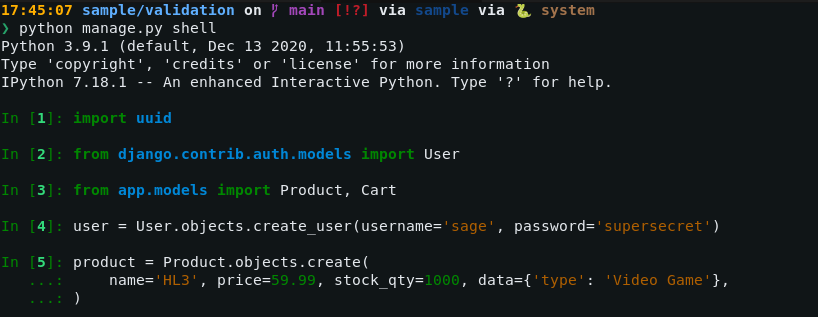
\includegraphics[width=0.90\textwidth]{pics/validation0.png}
	\caption{The initialization for the validation demonstration.}
	\label{fig:validation0}
\end{figure}

Before demonstrating the validators in action, some model objects are created,
as shown by \autoref{fig:validation0}. The first object is a \verb|User| object
that is assigned to the \verb|user| variable, which will be assigned to a
\verb|Cart| object. The second object is a \verb|Product| model object that is
assigned to the \verb|product| variable, which will be added to a \verb|Cart|
object. Both of these objects are created with the \verb|create()| method,
thus they are immediately saved to the database. After these objects are
created, the validators are demonstrated below.

\begin{figure}
	\centering
    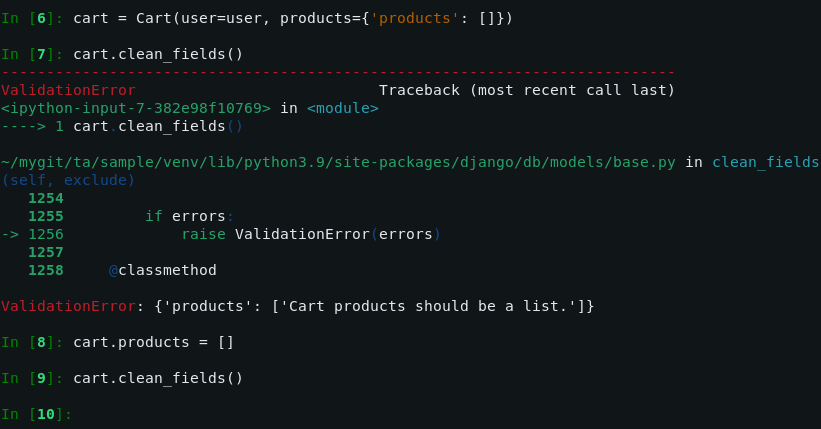
\includegraphics[width=0.90\textwidth]{pics/validation1.png}
	\caption{The \code{validate\_cart\_products\_list()} validator in action.}
	\label{fig:validation1}
\end{figure}

To run the validators before the \verb|Cart| model object is saved to the
database, an instance of the \verb|Cart| class is created (rather than using
the \verb|create()| method). The instance is linked to the \verb|user| created
previously and is initialized with the dictionary \verb|{'products': []}| as
the top-level value for the \verb|products| field. When calling the
\verb|clean_fields()| method, a \verb|ValidationError| is raised, as shown by
\autoref{fig:validation1}. The error message (that comes from the
\verb|validate_cart_products_list| validator) indicates that the
\verb|products| field value should be a \verb|list|, not a dictionary. After
changing the \verb|products| field's top-level value to an empty \verb|list|
(\verb|[]|), calling the \verb|clean_fields()| method again does not raise any
errors.

\begin{figure}
	\centering
    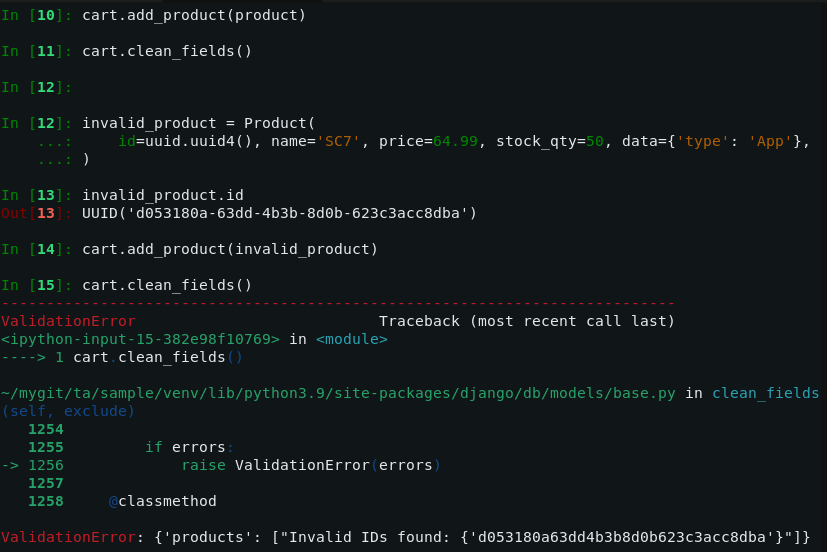
\includegraphics[width=0.90\textwidth]{pics/validation2.png}
	\caption{The \code{validate\_cart\_product\_ids\_exist} validator in action.}
	\label{fig:validation2}
\end{figure}

The next validator is the \verb|validate_cart_product_ids_exist()| function.
Before demonstrating this validator, the previously made \verb|product| object
is added to the \verb|cart|. If the \verb|clean_fields()| method is called, no
error is raised because the \verb|product| exists in the database, as shown by
input 11 of \autoref{fig:validation2}. After that, a new \verb|Product|
instance is created without saving it to the database (input 12). If the
instance is added to the \verb|cart| (input 14) and the \verb|clean_fields()|
method is called (input 15), a \verb|ValidationError| is raised. The error
message indicates that the invalid ID is equal to the new \verb|Product|
instance \verb|id| (input and output 13). The error is raised because the
new instance does not exist in the database yet.

\begin{figure}
	\centering
    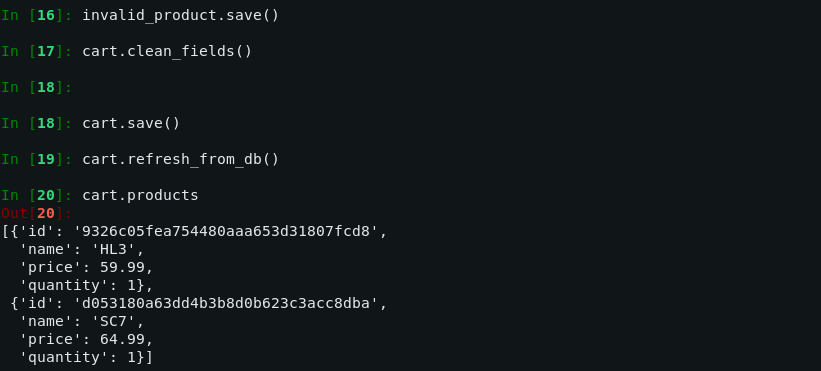
\includegraphics[width=0.90\textwidth]{pics/validation3.png}
	\caption{The \code{Cart} object is saved after passing the validations.}
	\label{fig:validation3}
\end{figure}

If the new \verb|Product| instance is saved, calling the \verb|clean_fields()|
method again does not raise an error, as shown by inputs 16 and 17 of
\autoref{fig:validation3}. As the list of \verb|products| in the \verb|cart|
has been validated, it can now be safely saved to the database. To save the
\verb|Cart| object, the \verb|save()| method is called (input 18). To verify
that the object is successfully saved, the \verb|refresh_from_db()| method is
called (input 19). As shown by input and output 20, the list of \verb|products|
were successfully stored to and retrieved from the database.

In this chapter, JSON data validation for a \verb|JSONField| has been
explained. The validation is implemented by creating custom validator functions
using and supplying them to the field using the \verb|validators| argument to
the field's constructor. To run the validators, the \verb|clean_fields()|
method of the field is called. If the data is not valid, the validators raise
\verb|ValidationError|s, which can be caught to prevent invalid data from being
saved to the database. In the next chapter, the \verb|JSONField| implementation
will be evaluated on multiple database systems.

\clearchapter
%-----------------------------------------------------------------------------%
\chapter{\babEnam}
%-----------------------------------------------------------------------------%

In this chapter, the \verb|JSONField| implementation explained in the fourth
chapter is evaluated on all of the database systems supported by Django.

%-----------------------------------------------------------------------------%
\section{Tests}
%-----------------------------------------------------------------------------%

To ensure that the behavior of \verb|JSONField| is consistent across all of the
database systems supported by Django, existing tests for the PostgreSQL-only
implementation are run for other database systems as well. The tests were
gradually moved from the \verb|postgres_tests| directory to the
\verb|model_fields| and \verb|form_tests/field_tests| directories during
development. By moving the tests outside of \verb|postgres_tests| and modifying
the test classes to use the new implementation, the tests can now be run on
other database systems.

\begin{table}
	\centering
\begin{tabular}{|c|l|c|p{6.6cm}|}
\hline
No. & Test class                  & No. of tests & Test cases description \\ \hline
1.  & \texttt{JSONFieldTests}     & 3            & Non-serializable value, custom encoder and decoder usage, and database \texttt{CHECK} constraints. \\ \hline
2.  & \texttt{TestMethods}        & 4            & \texttt{deconstruct()}, \texttt{get\_transforms()}, etc. \\ \hline
3.  & \texttt{TestValidation}     & 4            & Invalid encoder and decoder, invalid JSON value, etc. \\ \hline
4.  & \texttt{TestFormField}      & 2            & \texttt{formfield()} with and without custom encoder and decoder. \\ \hline
5.  & \texttt{TestSerialization}  & 2            & Serialization and deserialization with Django's serialization framework. \\ \hline
6.  & \texttt{TestSaveLoad}  	  & 6            & Saving and loading various JSON data. \\ \hline
7.  & \texttt{TestQuerying}       & 49           & Querying various JSON data with different scenarios (including lookups and transforms). \\ \hline
\end{tabular}
\caption{The \code{JSONField} model field test classes and their descriptions.}
\label{table:testclasses}
\end{table}

The tests for \verb|JSONField| are split into different files according to
Django's test files structure. The majority of the tests are written in the
\verb|model_fields.test_jsonfield| module, which consists of 70 test cases
divided into 7 test classes, as shown by \autoref{table:testclasses}. As seen
in the table, the \verb|JSONField| querying functionalities have the largest
number of tests for different querying scenarios. In addition to tests that
were moved from the PostgreSQL-only implementation, the \verb|JSONField| tests
also include new tests for new features and documented behaviors.

Aside from the tests specific to the model field, there are also tests for the
other parts of the ORM as well as the form field. The tests for the other ORM
parts include tests for system checks in regards to \verb|JSONField| support on
the database backends, tests for default value in \verb|JSONField|, tests for
\verb|JSONField| casting operations, and others. These tests are written in
separate modules, i.e. the \verb|test_models| and \verb|test_ordinary_fields|
modules in the \verb|invalid_models_tests| module, the
\verb|backends.base.test_operations| module, etc. Meanwhile, the form field
tests are written in the \verb|form_tests.field_tests.test_jsonfield| module,
which consists of 12 test cases in a single test class.

\listing
{Python}
{The \code{test\_custom\_encoder\_decoder()} test method.}
{code:testencodecoder}
{codes/6-testencodecoder.py}

One of the new tests is \verb|test_custom_encoder_decoder()| shown by
\autoref{code:testencodecoder}. The test is modified from
\verb|test_custom_encoder()| in the PostgreSQL-only implementation, which did
not support a custom decoder. The test describes the process of creating a
\verb|NullableJSONModel| object that contains a \verb|UUID| object inside a
\verb|JSONField| (lines 4 and 5). The \verb|NullableJSONModel| class is a model
class (for \verb|JSONField| tests) that has a \verb|JSONField| named
\verb|value_custom| that is equipped with custom encoder and decoder.  Upon
cleaning the fields (line 6) and saving the object to the database (line 7),
the object is retrieved (refreshed) from the database (line 8). The retrieved
object is asserted to be equal to the initial object (line 9), which means that
the JSON object is successfully deserialized to retain the \verb|UUID| object.
The deserialization is only possible if a custom decoder is used because the
default decoder does not provide deserialization to \verb|UUID| objects.

\listing
{Python}
{The \code{test\_json\_null\_different\_from\_sql\_null()} test method.}
{code:testnull}
{codes/6-testnull.py}

The \verb|test_json_null_different_from_sql_null()| method shown by
\autoref{code:testnull} is another example of the new tests. The test verifies
the \verb|JSONField| behavior with JSON \verb|null| and SQL \verb|NULL| values,
which was not documented in the PostgreSQL-only implementation. The test works
by using JSON \verb|null| and SQL \verb|NULL| values to create model objects
that are assigned to \verb|json_null| and \verb|sql_null| variables,
respectively (lines 5 and 7). After refreshing both objects (lines 6 and 8),
queries for the JSON \verb|null| value is verified using \verb|Value('null')|
and \verb|None| (lines 10 to 17). Meanwhile, the SQL \verb|NULL| value is
verified by using the \verb|isnull| lookup (lines 18 to 21). Finally, both
values are asserted to be equal in Python, i.e. \verb|None|.

\begin{figure}
	\centering
    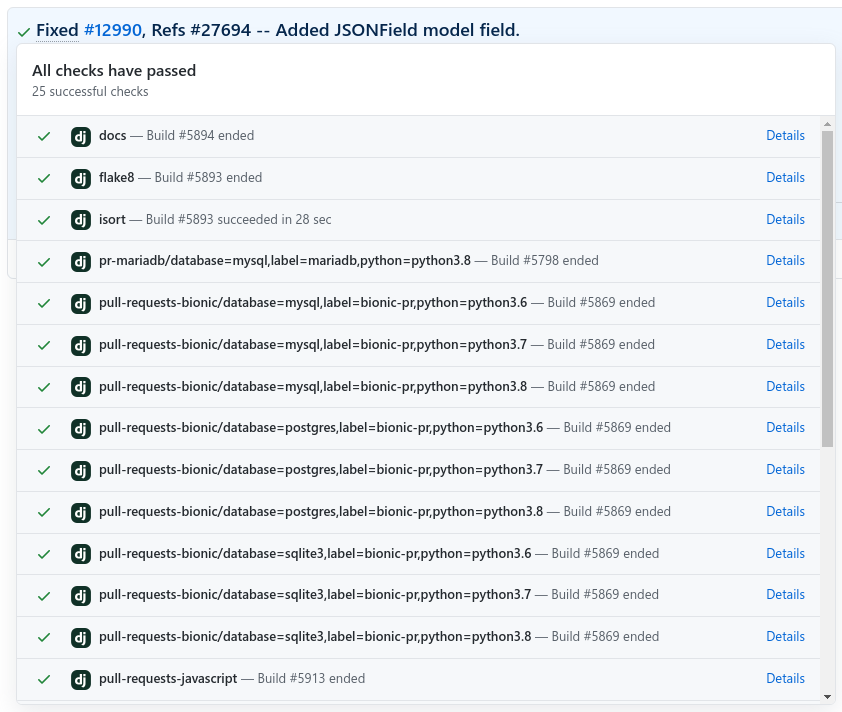
\includegraphics[width=1.00\textwidth]{pics/github-checks.png}
	\caption{The tests have passed on all of the database systems
	(Oracle Database not shown).}
	\label{fig:checks}
\end{figure}

At the time of research, the tests were run on all database systems and Python
3.6, 3.7, and 3.8. The tests were run on Django's Jenkins
instance\footnote{\url{https://djangoci.com}} and the summary that shows the
tests have passed on all database systems can be seen on
GitHub\footnote{\url{https://github.com/django/django/commit/6789ded0a6ab797f0dcdfa6ad5d1cfa46e23abcd}},
as shown by \autoref{fig:checks}. For Oracle Database, the tests have to be
triggered manually by the Django maintainers. In the final version of the Git
commit, the maintainers did not trigger the tests for Oracle Database, hence
the result cannot be seen in \autoref{fig:checks}. Unfortunately, the build
details and logs for the commit (and the previous iterations) could no longer
be retrieved from the Jenkins instance at the time of writing.

The tests for the new \verb|JSONField| have incorporated the tests from the
previous PostgreSQL-only implementation. Passing the tests means that the new
implementation retains the functionalities of the previous implementation.
To avoid redundancy, the PostgreSQL-only implementation is deprecated and
programmers are advised to use the new implementation instead. The deprecation
will be explained in the next section.

%-----------------------------------------------------------------------------%
\section{Deprecation of the PostgreSQL-only \code{JSONField}}
%-----------------------------------------------------------------------------%

Django has a deprecation policy that should be followed when deprecating the
PostgreSQL-only \verb|JSONField| implementation
\cite{django:deprecation-policy}. According to the policy and the deprecation
guide, the release of Django 3.1 should contain a backwards-compatible replica
of the field that raises a \verb|RemovedInDjango40Warning|
\cite{django:deprecation-guide}. The replica will still be included in the
Django 3.2 release, but it will be removed in the Django 4.0 release.

\listing
{Python}
{The deprecated \code{JSONField} model field.}
{code:depjsonfield}
{codes/6-depjsonfield.py}

The \verb|JSONField| model field in the
\verb|django.contrib.postgres.fields.jsonb| module is now deprecated and
replaced with a backwards-compatible replica shown by
\autoref{code:depjsonfield}. The replica is created by extending the new
\verb|JSONField| (imported as \verb|BuiltinJSONField|) without overriding any
methods. Thus, the replica works the same way as the new implementation. The
only differences between the two are the module locations and the
\verb|system_check_deprecated_details| property defined in the replica (lines 2
to 10), which makes the replica raise a system check warning on initialization.
The warning includes a hint to use the \verb|django.db.models.JSONField| class
instead (line 8). The Django developers assigned the warning \verb|id| to be
\verb|fields.W904| (line 9).

\listing
{Python}
{The deprecated \code{JSONField} form field.}
{code:depformfield}
{codes/6-depformfield.py}

The \verb|JSONField| form field in the
\verb|django.contrib.postgres.forms.jsonb| is also deprecated and replaced with
a replica shown by \autoref{code:depformfield}. As with the model field, the
replica is created by extending the new \verb|JSONField| form field without
overriding any methods. However, unlike the model field, the base \verb|Field|
class for form fields does not use the \verb|system_check_deprecated_details|
property. Therefore, the warning is raised explicitly in the constructor by
calling \verb|warnings.warn|, as shown by lines 2 to 7 of the listing. The
\verb|RemovedInDjango40Warning| class is used as the \verb|category| argument
of \verb|warnings.warn|, as shown by line 6.

\listing
{Python}
{The deprecated \code{KeyTransform} and \code{KeyTextTransform}.}
{code:deptransforms}
{codes/6-deptransforms.py}

In addition to the \verb|JSONField| model and form fields, the transform
classes are also deprecated and replaced with replicas shown by
\autoref{code:deptransforms}. The replicas are needed because there are use
cases (covered in tests) that need the classes to be instantiated directly. As
with the form field, the replicas are created by extending the classes from the
new implementation. The system warnings are also raised explicitly in the
constructor, as shown by the calls to \verb|warnings.warn| in the listing.

Unlike the \verb|KeyTransform| and \verb|KeyTextTransform| classes, the lookup
classes of the PostgreSQL-only implementation are deprecated by removing them.
The reason for the removal is that the classes are not meant to be instantiated
directly. Instead, the classes are meant to be used with the
\verb|__lookup_name| syntax as keyword arguments in the QuerySet API. The
classes from the previous implementation can safely be removed because the
lookups are already registered in the new implementation of the model field, so
the replica also has the lookups registered.

By replacing the PostgreSQL-only fields and transforms with the replicas, the
deprecation is now complete. The tests described in the previous section also
guarantee the new implementation to be compatible with the previous
PostgreSQL-only implementation. Thus, backward compatibility is preserved and
programmers will be notified to update their code. With the deprecation and
tests written, the goals of this research have been completed. Therefore, the
next chapter will discuss the conclusions of this research.

\clearchapter
%---------------------------------------------------------------
\chapter{\kesimpulan}
%---------------------------------------------------------------
This chapter discusses the conclusions of this research and suggestions for
future research.

%---------------------------------------------------------------
\section{Conclusions}
%---------------------------------------------------------------

The primary objective of this research is to implement a new \verb|JSONField|
that can be used on all database backends supported by Django. The
\verb|JSONField| implementation includes the model field, form field, lookups,
and transforms. The implementation should handle the differences in how JSON
data is managed by all of the database systems, which consist of PostgreSQL,
MariaDB, MySQL, SQLite, and Oracle Database.

To handle the differences between the database systems, some adjustments to the
database backends were needed. The adjustments included the additions of new
feature flags in the \verb|DatabaseFeature| classes of the database backends.
The flags indicate the different behaviors of each database system, which can
be used to determine how the implementation on the database system should be
created. Some adjustments were also made to the \verb|DatabaseWrapper| classes
to define the data types and SQL \verb|CHECK| constraints on the database
level. Some database backends also require some adjustments to the
\verb|DatabaseOperations| class to define some casting operations for JSON
data.

After creating the database backend adjustments, \verb|JSONField| and its
lookups and transforms could be implemented. The \verb|JSONField| model field
was implemented by serializing the data before it is sent to the database and
deserializing the data when it is retrieved from the database. On the other
hand, the \verb|JSONField| form field could be used without any modifications
as it does not interact with the database directly. Both the model field and
form fields were updated to support custom encoder and decoder for
serialization and deserialization. The lookups and transforms were implemented
by utilizing the JSON functions that are available on the database systems.

The secondary objective of this research is to provide examples of how
validation rules can be applied to a \verb|JSONField|. For demonstration, a
small Django project with an e-commerce scenario was created. The project
includes two models, \verb|Product| and \verb|Cart|, that represent a product
and a shopping cart on an e-commerce website. The \verb|Cart| model has a
\verb|JSONField| that uses validators to validate the data. The validators were
added using the validation feature in Django. By utilizing the validators, JSON
data in a model field could be validated by calling the \verb|clean_fields()|
method of the model instance and catching the \verb|ValidationError| exception.

To ensure that the new implementation of \verb|JSONField| is consistent on all
database backends, \verb|JSONField| tests were run on all database systems. The
tests included test cases for the new features and documented behaviors, such
as the custom decoder support and the \verb|JSONField| behavior when handling
JSON \verb|null| and SQL \verb|NULL| values. In addition, the \verb|JSONField|
tests also incorporated the tests from the previous PostgreSQL-only
implementation to ensure that backward compatibility is preserved. After
passing the tests, the previous implementation was deprecated by creating
replicas of the classes and raising system warnings about the deprecation.

%---------------------------------------------------------------
\section{Suggestions}
%---------------------------------------------------------------
Based on the results of this research, some suggestions for future research are
as follow:

\begin{enumerate}
	\item The Query Expression API in Django supports a variety of use cases
		  through the use of built-in and custom query expressions. While the
		  tests in this research have included the common use cases, it is not
		  feasible to test each and every possible use case with
		  \verb|JSONField|. In addition, the \verb|JSONField| implementation in
		  this research has not yet supported efficient partial updates to JSON
		  data using the \verb|update()| method of the QuerySet API. Thus, more
		  complex use cases of \verb|JSONField| with Django's ORM tool on all
		  database backends may be a subject of future research.
	\item This research has provided some examples of JSON data validation,
		  including a basic example of how the schema of a \verb|JSONField| can
		  be validated. For more complex schemas, third-party packages can be
		  utilized to create the validation rules. Integrating the third-party
		  packages with Django's validators may be explored in future
		  research.
	\item Recent studies have shown interest in measuring the performance of
		  relational databases in handling JSON data. Relational databases are
		  not dedicated for storing JSON data, thus they may not perform well
		  compared to NoSQL databases. However, recent benchmarks have shown
		  that a relational database system could outperform a NoSQL database
		  system in varied workloads with JSON data
		  \cite{enterprisedb_benchmark}. Some extensive benchmarks on multiple
		  database systems have also shown that the performance differences
		  between relational and NoSQL databases were not significant,
		  especially for smaller documents \cite{dolgov_benchmark}. However,
		  these benchmarks were done directly on the database systems instead
		  of using an ORM tool. Therefore, further research on relational
		  databases' performance in handling JSON data using an ORM tool such
		  as \verb|JSONField| would provide new insights on this topic.
\end{enumerate}

\clearchapter

%
% Daftar Pustaka
%
% Daftar Pustaka
%

%
% Tambahkan pustaka yang digunakan setelah perintah berikut.
%
\phantomsection %hack to add clickable section for pustaka
\printbibliography

\clearchapter

%
% Lampiran
%
% \begin{appendix}
% 	%
% @author  Andreas Febrian
% @version 1.00
%
% Hanya sebuah pembatas bertuliskan LAMPIRAN ditengah halaman.
%

\begin{titlepage}
	\centering
	\vspace*{6cm}
	\noindent \Huge{LAMPIRAN}
	\addChapter{LAMPIRAN}
\end{titlepage}

% 	\clearchapter
% 	\setcounter{page}{2}
% 	%-----------------------------------------------------------------------------%
\addChapter{Lampiran 1: Judul Lampiran 1}
\chapter*{Lampiran 1: Judul Lampiran 1}
%-----------------------------------------------------------------------------%
Lampiran hadir untuk menampung hal-hal yang dapat menunjang pemahaman terkait tugas akhir, namun akan mengganggu \f{flow} bacaan sekiranya dimasukkan ke dalam bacaan.
Lampiran bisa saja berisi data-data tambahan, analisis tambahan, penjelasan istilah, tahapan-tahapan antara yang bukan menjadi fokus utama, atau pranala menuju halaman luar yang penting.

%-----------------------------------------------------------------------------%
\section*{Subbab dari Lampiran 1}
%-----------------------------------------------------------------------------%
\todo{Isi subbab ini sesuai keperluan Anda. Anda bisa membuat lebih dari satu judul lampiran, dan tentunya lebih dari satu subbab.}

% \end{appendix}

\end{document}
